%%%%%%%%%%%%%%%%%%%% author.tex %%%%%%%%%%%%%%%%%%%%%%%%%%%%%%%%%%%
%
% sample root file for your "contribution" to a contributed volume
%
% Use this file as a template for your own input.
%
%%%%%%%%%%%%%%%% Springer %%%%%%%%%%%%%%%%%%%%%%%%%%%%%%%%%%


% RECOMMENDED %%%%%%%%%%%%%%%%%%%%%%%%%%%%%%%%%%%%%%%%%%%%%%%%%%%
\documentclass[graybox]{svmult}

% choose options for [] as required from the list
% in the Reference Guide

\usepackage{mathptmx}       % selects Times Roman as basic font
\usepackage{helvet}         % selects Helvetica as sans-serif font
\usepackage{courier}        % selects Courier as typewriter font
\usepackage{type1cm}        % activate if the above 3 fonts are
                            % not available on your system
%
\usepackage{makeidx}         % allows index generation
\usepackage{graphicx}        % standard LaTeX graphics tool
                             % when including figure files
\usepackage{multicol}        % used for the two-column index
\usepackage[bottom]{footmisc}% places footnotes at page bottom

\usepackage{qtree, bm, amsmath, amssymb, qtree, bm, multirow, textcmds, siunitx, mathrsfs, float, booktabs, color, soul}
\usepackage{natbib, setspace}
\usepackage{pdfpages} %To insert pdf pages
\usepackage[bb=boondox]{mathalfa}
\usepackage{tikz}
\definecolor{hfill_blue}{RGB}{208,229,249}
\definecolor{hfill_yellow}{RGB}{255,255,208}
\usetikzlibrary{trees,shapes}
\usetikzlibrary{matrix}
\tikzstyle{line} = [draw, thick]

% see the list of further useful packages
% in the Reference Guide

\makeindex             % used for the subject index
                       % please use the style svind.ist with
                       % your makeindex program

%%%%%%%%%%%%%%%%%%%%%%%%%%%%%%%%%%%%%%%%%%%%%%%%%%%%%%%%%%%%%%%%%%%%%%%%%%%%%%%%%%%%%%%%%
%\textsc{\textsc{\bibliographystyle{natbb}
%
%\bibliography{References_HTSF}

\def\ba{\begin{pmatrix}\tilde{\vec{b}}\\ \tilde{\vec{a}}\end{pmatrix}}
\def\GH{\begin{pmatrix}\vec{G}\\ \vec{F}\end{pmatrix}}
\def\Naive{Na\"{i}ve\ }
\def\naive{na\"{i}ve\ }



\begin{document}

\title*{Hierarchical Forecasting}
% Use \titlerunning{Short Title} for an abbreviated version of
% your contribution title if the original one is too long
\author{Name of First Author and Name of Second Author}
% Use \authorrunning{Short Title} for an abbreviated version of
% your contribution title if the original one is too long
\institute{Name of First Author \at Name, Address of Institute, \email{name@email.address}
\and Name of Second Author \at Name, Address of Institute \email{name@email.address}}
%
% Use the package "url.sty" to avoid
% problems with special characters
% used in your e-mail or web address
%
\maketitle

\abstract*{TBC}


\section{Introduction}\label{sec:intro}


\begin{itemize}
	\item Importance of coherency
	\item Point forecasting
	\item Probabilistic forecasting
\end{itemize}
			

The key macroeconomic indicators such as Gross Domestic Product (GDP), inflation and monetary policies which are used to study the behavior and performance of an economy as a whole are it self aggregates of various other components.
For example, if we take the GDP growth, it is the aggregate of consumption, government expenditure, investments and net exports. These four components are again aggregates of some sub components. When we collect data for each of these individual variab
les over some time period, we will observe a collection of multiple time series that are bounded with some aggregation constraints. Thus the macroeconomic data are naturally forming cross sectional hierarchical time series.

If the interest is on a single macroeconomic variable along different time granularities, then it can be considered as a temporal hierarchy. For example, suppose we have monthly consumer product index (CPI) of a particular country. The quarterly CPI is then the aggregate of corresponding monthly CPI of each quarter. Similarly the yearly CPI is the aggregate of quarterly CPI of each year. Hence it will form a temporal hierarchy.

Macroeconomic forecasts are crucial for economic and business activities of any economy. Therefore this area of study has a long history in literature. Econometricians have developed various approaches for getting reliable economic forecasts using macroeconomic data. However, the information of aggregation structure in real data is limitedly used in literature. Moreover, having coherent forecasts will help the economists and policy makers for align decision making that impact for the whole economy. Therefore, our focus in this chapter is to introduce hierarchical forecasting methods for macroeconomic forecasting particularly for cross-sectional hierarchical data structures.

Obtaining coherent forecasts are independent from the forecasting models. That means forecasters were given the freedom to use any reliable forecasting method to obtain the forecasts for individual series in the hierarchy. Getting coherent forecasts is a post-processing technique which ensures the aggregation properties are preserved in the forecasts.   \\


\textcolor{red}{briefly discuss the point forecasts as well as probabilistic forecasts in the sense of macroeconomic data  }

\begin{itemize}
	\item Importance of coherency
	\item Point forecasting
	\item Probabilistic forecasting
\end{itemize}
\clearpage
\section{Hierarchical time series}\label{sec:Hier ts}

\textcolor{red}{Fix this depending on Section 2} To simplify the introduction of some notation we use the simple two-level hierarchical structure shown in Figure \ref{fig:simple tree}. Denote as $y_{Tot,t}$ the value observed at time $t$ for the most aggregate (Total) series  corresponding to level 0 of the hierarchy. Below level 0, denote as $y_{i,t}$ the value of the series corresponding to node $i$, observed at time $t$. For example, $y_{A,t}$ denotes the $t$th observation of the series corresponding to node A at level 1, $y_{AB,t}$ denotes the $t$th observation of the series corresponding to node AB at level 2, and so on.

\begin{figure}[!hbt]  \center
  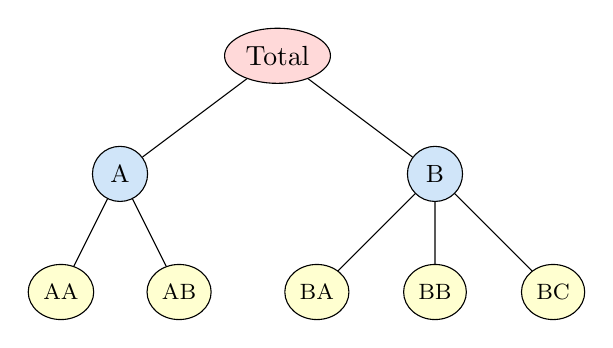
\begin{tikzpicture}
    \tikzstyle{every node}=[ellipse,draw,inner sep=2pt,minimum size=7mm,fill=red!15] %158,202,225
    \tikzstyle[level distance=.1cm]
    \tikzstyle[sibling distance=.1cm]
    %\tikzstyle{level 3}=[sibling distance=6.2mm,font=\tiny]
    \tikzstyle{level 1}=[sibling distance=40mm, font=\small, set style={{every node}+=[fill=hfill_blue]}]
    \tikzstyle{level 2}=[sibling distance=15mm, font=\footnotesize, set style={{every node}+=[fill=hfill_yellow]}]
    \node{Total}%[edge from parent fork down]
    child {node {A}
      child {node {AA}}
      child {node {AB}}
    }
    child {node {B}
      child {node {BA}}
      child {node {BB}}
      child {node {BC}}
    };
  \end{tikzpicture}
  \caption{A simple two-level hierarchical structure.}
  \label{fig:simple tree}
\end{figure}

Let $\vec{y}_t = (y_{Tot,t},y_{A,t}, y_{B,t},y_{AA,t}, y_{AB,t}, y_{BA,t}, y_{BB,t},y_{BC,t})'$, a vector containing observations across all series of the hierarchy at $t$. Similarly denote as \linebreak $\vec{b}_t = (y_{AA,t}, y_{AB,t}, y_{BA,t}, y_{BB,t}, y_{BC,t})'$ a vector containing observations only for the bottom-level series. In general, $\vec{y}_t\in \mathbb{R}^n$ and $\vec{b}_t \in \mathbb{R}^m$ where $n$ denotes the number of total series in the structure, $m$ the number of series at the bottom level, and $n>m$ always. In the simple example of Figure \ref{fig:simple tree}, $n=8$ and $m=5$.

Aggregation constraints dictate that $y_{Tot}=y_{A,t}+y_{B,t}=y_{AA,t}+y_{AB,t}+y_{BA,t}+y_{BB,t}+y_{BC,t}$,~ $y_{A,t}=y_{AA,t}+y_{AB,t}$ and $y_{B}=y_{BA,t}+y_{BB,t}+y_{BC,t}$. Hence we can write
\begin{equation}\label{eq:summing matrix}
\vec{y}_t = \vec{Sb}_t,
\end{equation}
where \begin{equation*}
\vec{S} = \begin{pmatrix}
1& 1& 1& 1 & 1 \\
1& 1& 0& 0 & 0\\
0& 0& 1& 1 & 1\\
& \multicolumn{3}{c}{\vec{I}_5} &
\end{pmatrix}
\end{equation*}
an $n\times m$ matrix referred to as the \textit{summing matrix} and $\vec{I}_m$ is an $m$-dimensional identity matrix. $\vec{S}$ reflects the linear aggregation constraints and in particular how the bottom-level series aggregate to levels above. Thus, columns of $\vec{S}$ span the linear subspace of $\mathbb{R}^n$ for which the aggregation constraints hold. We refer to this as the \textit{coherent subspace} and denote it by $\mathfrak{s}$. Notice that pre-multiplying a vector in $\mathbb{R}^m$ by $\vec{S}$ will result in an $n$-dimensional vector that lies in $\mathfrak{s}$.

\begin{property}
A hierarchical time series has observations that are \textit{coherent}, i.e., $\vec{y}_{t} \in \mathfrak{s}$ for all $t$. We use the term coherent to describe not just $\vec{y}_t$ but any vector in $\mathfrak{s}$.
  \label{def:coherence}
\end{property}


Structures similar to the one portrayed in Figure \ref{fig:simple tree} can be found in macroeconomics. For instance in Section~\ref{XXX} we consider the case of GDP and its components.  However, while this motivating example involves aggregation constraints, the mathematical framework we use can be applied for any general linear constraints, examples of which are ubiquitous in macroeconomics. For instance, the trade balance is computed as exports minus imports, while the consumer price index is computed as a weighted average of sub-indices, which are in turn weighted averages of sub-sub-indices and so on.  These structures can also be captured by an appropriately designed $\vec{S}$ matrix.

An important alternative aggregation structure also commonly found in macroeconomics, is one for which the most aggregate series is disaggregated by attributes of interest that are crossed, as distinct to nested which is the case for hierarchical time series. For example, industrial production may be disaggregated along the lines of geography or sector or both. We refer to this as a \textit{grouped} structure. Figure \ref{fig:simple grouped tree} shows a simple example of such a structure. The Total series disaggregates into $y_{A,t}$ and $y_{B,t}$, but also into $y_{X,t}$ and $y_{Y,t}$, at level 1, and then into the bottom-level series, $\vec{b}_t=(y_{AX}, y_{AY}, y_{BX}, y_{BY})'$. Hence, in contrast to hierarchical, grouped time series do not naturally disaggregate in a unique manner.
\begin{figure}[!hbt]
\center
\tikzstyle{every node}=[inner sep=2pt,minimum size=7mm]
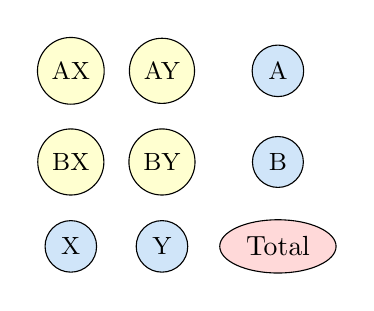
\begin{tikzpicture}
    \matrix[ampersand replacement=\&,column sep=0.3cm] {
        \node[circle,draw,fill=hfill_yellow, font=\small,distance=1cm] {AX};~ \&
        \node[circle,draw,fill=hfill_yellow,font=\small] {AY};~ \&
        \node[circle,draw,fill=hfill_blue, font=\small] {A}; \\[0.3cm]
        \node[circle,draw,fill=hfill_yellow, font=\small] {BX};~ \&
        \node[circle,draw,fill=hfill_yellow, font=\small] {BY};~ \&
        \node[circle,draw,fill=hfill_blue, font=\small] {B}; \\[0.3cm]
        \node[circle,draw,fill=hfill_blue, font=\small] {X};~ \&
        \node[circle,draw,fill=hfill_blue, font=\small] {Y};~ \&
        \node[ellipse,draw,fill=red!15] {Total}; \\
};
\end{tikzpicture}
  \caption{A simple two-level grouped structure.}
  \label{fig:simple grouped tree}
\end{figure}

An important implementation of aggregation structures are \textit{temporal hierarchies} introduced by \cite{AthEtAl2017}. In this case the aggregation structure spans the time dimension and dictates how higher frequency data (e.g., monthly) are aggregated to lower frequencies. There is a vast literature that studies the effects of temporal aggregation, going back to the seminal work of \cite{ZelMon1971, AmeWu1972, Tia1972, Bre1973} and others such as, \cite{Hot1993, HotCar1993, Mar1999, SilEtAl2008}. The main aim of this work is to find the single most optimum level of aggregation for modelling and forecasting time series. In this literature, the analyses, results (whether theoretical or empirical) and inferences, are extremely heterogeneous, making it very challenging to reach a consensus or some concrete conclusions. For example, \cite{RosSea1995} who study the effect of aggregation on several key macroeconomic variables state, ``Quarterly data do not seem to suffer badly from temporal aggregation distortion, nor are they subject to the construction problems affecting monthly data. They therefore may be the optimal data for econometric analysis.'' A similar conclusion is reached by \cite{NijPal1990}. \cite{SilEtAl2008} consider forecasting French cash state deficit and provide empirical evidence of forecast accuracy gains from forecasting with the aggregate model rather than aggregating forecasts from the disaggregate model.

The overwhelming majority of the literature concentrates on a single level of temporal aggregation \citep[there are some notable exceptions such as,][]{AndEtAl2011,KouEtAl2014}. \cite{AthEtAl2017} show that considering multiple levels of aggregation via temporal hierarchies and implementing forecast reconciliation approaches rather than single level approaches results in substantial gains in forecast accuracy across all levels of temporal aggregation. This is an example of the benefits of forecast reconciliation to which we now turn out attention to.

\section{Point forecasting}\label{sec:point forecasting}

A requirement when forecasting hierarchial time series is that the forecasts adhere to the same aggregation constraints as the observed data, i.e., they are coherent.

\begin{definition}
A set of $h$-step ahead forecasts $\tilde{\vec{y}}_{T+h|T}$, stacked in the same order as $\vec{y}_{t}$ and generated using information up to and including time $T$,
are said to be \textit{coherent} if $\tilde{\vec{y}}_{T+h|T} \in \mathfrak{s}$.
  \label{def:coherence}
\end{definition}

Hence, coherent forecasts of lower level series aggregate up to their corresponding upper level series and vice versa.

\textcolor{red}{Add the picture here.}
Let us consider the smallest possible hierarchy with two bottom level series, $A$ and $B$ that add up to the top level $Tot$. Suppose $\breve{\vec{y}}_{T+h|T}$ of this hierarchy is given by $\breve{\vec{y}}_{T+h|T} = [\breve{y}_{Tot,T+h|T},\breve{y}_{A,T+h|T}, \breve{y}_{B,T+h|T}]$. Due to the aggregation structure we have $\breve{y}_{Tot,T+h|T}=\breve{y}_{A,T+h|T}+\breve{y}_{B,T+h|T}$. This implies that, even though  $\breve{\vec{y}}_{Tot,T+h|T} \in \mathbb{R}^3$, the points actually lie in $\mathfrak{s}\subset \mathbb{R}^3$, which is a two dimensional subspace within $\mathbb{R}^3$ space.

\subsection{Single-level approaches}\label{sec:single level approaches}
A common theme across all traditional approaches for forecasting hierarchical time series is that a single-level of aggregation is first selected and forecasts for that level are generated. These are then linearly combined to generate a set of coherent forecasts the rest of the structure.

\subsubsection{Bottom-up}

In the \textit{bottom-up} approach, forecasts for the most disaggregate are first generated. These are then aggregated to obtain forecasts for all other series of the hierarchy \citep{dunn1976}. In general, this consists of first generating $\hat{\vec{b}}_{T+h|T} \in \mathbb{R}^m$, a set of $h$-step ahead forecasts for the bottom-level series. For the simple hierarchical structure of Figure \ref{fig:simple tree}, $\hat{\vec{b}}_{T+h|T} = (\hat{{y}}_{AA,T+h|T}, \hat{{y}}_{AB,T+h|T}, \hat{{y}}_{BA,T+h|T}, \hat{{y}}_{BB,T+h|T},\hat{{y}}_{BC,T+h|T}),$ where, $\hat{{y}}_{i,T+h|T}$ is the $h$-step ahead forecast of the series corresponding to node $i$. A set of coherent forecasts for the whole hierarchy is then given by,
\begin{equation*}\label{eq:BU}
\tilde{\vec{y}}^{BU}_{T+h|T}=\vec{S\hat{\vec{b}}}_{T+h|T}.
\end{equation*}
Generating bottom-up forecasts has the advantage of no information being lost due to aggregation. However, bottom-level data can potentially be highly volatile or very noisy and therefore challenging to forecast.

\subsubsection{Top-down}

In contrast \textit{top-down} approaches involve first generating forecasts for the most aggregate level and then disaggregating these down the hierarchy. In general, coherent forecasts generated from top-down approaches are given by,
\begin{equation*}
\tilde{\vec{y}}^{TD}_{T+h|T}=\vec{S}\vec{p}\hat{y}_{Tot, T+h|T},
\end{equation*}
where $\vec{p} = (p_1,...,p_m)'$ is an $m$-dimensional vector consisting of a set of proportions which disaggregate the top-level forecast $\hat{y}_{Tot, T+h|T}$ to forecasts for the bottom-level series, hence $\vec{p}\hat{y}_{Tot, T+h|T}=\vec{\hat{\vec{b}}}_{T+h|T}$. These are then aggregated up by the summing matrix $\vec{S}$.

Traditionally proportions have been calculated based on the observed historical data. \cite{gross1990} present and evaluate twenty-one alternative approaches. The most convenient attribute of these approaches is their simplicity. Generating a set of coherent forecasts involves only modelling and generating forecasts for the most aggregate top-level series. In general, such top-down approaches seem to produce quite reliable forecasts for the aggregate levels and they are useful with low count data. However, a significant disadvantage is the loss of information due to aggregation. Using such top-down approaches, is limited as it does not allow to capture and model individual series characteristics. To overcome this limitation, \cite{AthEtAl2009} introduced a new top-down approach which disaggregates the top-level forecasts based on proportions of forecasts rather than the historical data and show evidence that this method outperforms the conventional top-down approaches. However, a limitation of all top-down and by implication middle-out approaches that follow next, is that they introduce bias to the forecasts. We discuss this in detail in Section \ref{sec:reconciliation approaches} that follows.

\subsubsection{Middle-out}

A compromise between bottom-up and top-down approaches is the middle-out approach. It entails first forecasting the series of a selected middle-level. For series above the middle-level, coherent forecasts are generated using the bottom-up approach by aggregating the middle-level forecasts upwards. For series below the middle level, coherent forecasts are generated using a top-down approach by disaggregating the middle-level forecasts downwards. As mentioned above As the since the middle-out approach involves generating top-down forecasts, it also introduces bias to the forecasts. We discuss this in detail in Section \ref{sec:reconciliation approaches} that follows.



\subsection{Point forecast reconciliation}\label{sec:reconciliation approaches}

All approaches discussed so far are limited to only using information from a single-level of aggregation. Furthermore, these ignore any correlations across levels of a hierarchy. An alternative framework that overcomes these limitations is one that involves forecast \textit{reconciliation}. In a first step ignoring any aggregation constraints, forecasts for all the series across all levels of the hierarchy are generated. We refer to these as \textit{base} forecasts and denote them by $\hat{\vec{y}}_{T+h|T}$. In general, base forecasts will not be coherent. An example of an exception is when a simple method such as a random walk is used to generate \naive base forecasts for all the series in the hierarchy. In this case coherent nature of the data is extended to the forecasts.

In a second step, base forecasts are reconciled, in an ex-post adjustment, so that they become coherent. This is achieved by projecting the base forecasts $\hat{\vec{y}}_{T+h|T}$ onto the coherent subspace $\mathfrak{s}$, via a projection matrix $\vec{SG}$, resulting in a set of coherent forecasts $\tilde{\vec{y}}_{T+h|T}$. More specifically,
\begin{equation}\label{eq:recon}
\tilde{\vec{y}}_{T+h|T}=\vec{S}\vec{G}\hat{\vec{y}}_{T+h|T},
\end{equation}
where $\vec{G}$ is an $m\times n$ matrix that maps $\hat{\vec{y}}_{T+h|T}$ to the $\mathbb{R}^m$ space, producing a set of coherent forecasts for the bottom-level which are in turn mapped to the coherent subspace by the summing matrix $\vec{S}$ as defined in \eqref{eq:summing matrix}. We restrict our attention to projections on $\mathfrak{s}$ in which case $\vec{SGS}=\vec{S}$. This ensures that unbiasedness is preserved, i.e., for a set of unbiased base forecasts reconciled forecasts will also be unbiased.



Note that all single-level approaches discussed so far can also be represented by \eqref{eq:recon} using appropriately designed \vec{G} matrices, however not all of these will be projections. For example, for the bottom-up approach, $\vec{G}=\begin{pmatrix}
\vec{0}_{(m \times n-m)} & \vec{I}_m
\end{pmatrix}$ in which case $\vec{SGS}=\vec{S}$. For any top-down approach
$\vec{G}=\begin{pmatrix}
\vec{p} & \vec{0}_{(m \times n-1)}
\end{pmatrix}$, for which case $\vec{SGS}\ne\vec{S}$.


\subsubsection{Optimal MinT reconciliation}

\cite{WicEtAl2019} build a unifying framework for much of the previous literature on forecast reconciliation. WE PRESENT THIS HERE AND LINK IT TO OTHER PAPERS

Assume that $\hat{\vec{y}}_{T+h|T}$ is a set of unbiased base forecasts, i.e., $E_{1:t}(\hat{\vec{y}}_{T+h|T})= E_{1:t}[\vec{y}_{T+h}|\vec{y}_1,...,\vec{y}_T]$, the true mean with the expectation taken over the observed sample up to time $T$.
Let
\begin{equation}\label{eq:base errors}
\hat{\vec{e}}_{T+h|T} = \vec{y}_{T+h|T}-\hat{\vec{y}}_{T+h|T}
\end{equation}
denote a set of base forecast errors with Var$(\hat{\vec{e}}_{T+h|T})=\vec{W}_h$, and
\begin{equation*}
\tilde{\vec{e}}_{T+h|T} = \vec{y}_{T+h|T}-\tilde{\vec{y}}_{T+h|T}
\end{equation*} denote a set of coherent forecast errors. Lemma 1 in \cite{WicEtAl2019} shows that for any matrix $\vec{G}$ such that $\vec{S}\vec{G}\vec{S}=\vec{S}$, $\text{Var}(\tilde{\vec{e}}_{T+h|T})=\vec{S}\vec{G}\vec{W}_h\vec{S}'\vec{G}'
$. Furthermore Theorem 1 shows that
\begin{equation} \label{eq:MinT}
\vec{G} = (\vec{S}'{\vec{W}}^{-1}_h\vec{S})^{-1}\vec{S}'{\vec{W}}^{-1}_h
\end{equation}
is the unique solution that minimises the tr$[\vec{S}\vec{G}\vec{W}_h\vec{S}'\vec{G}']$ subject to $\vec{S}\vec{G}\vec{S}=\vec{S}$. MinT is optimal in the sense that given a set of unbiased base forecasts, it returns a set of best linear unbiased reconciled forecasts using as $\vec{G}$ the unique solution that minimises the trace (hence MinT) of the variance of the forecast error of the reconciled forecasts. A significant advantage of the MinT reconciliation solution is that it is the first to incorporate the full correlation structure of the hierarchy via ${\vec{W}}_{h}$. However, estimating ${\vec{W}}_{h}$ is challenging, especially for $h>1$. \citet{WicEtAl2019} present possible alternative estimators for ${\vec{W}}_{h}$ and show that these lead to different $\vec{G}$ matrices. We summarise these below.


Note that unlike the GLS solution to \eqref{eq:OLS}, the MinT solution is a function of $\vec{W}_h$, the variance of the base forecast errors.


Of course setting ${\vec{W}}_{h}=k_h\vec{I}_n$ for all $h$ where $k_h>0$ is a proportionality constant, leads to the OLS solution of \cite{HynEtAl2011}. A disadvantage of this simplifying solution, further to not accounting for the correlations across series, is that the homoscedastic diagonal entries do not account for the scale differences between the levels of the hierarchy due to aggregation. \textcolor{red}{However OLS does well in practice because as discussed it minimises the Euclidean distance and blah blah. Not sure how much we want to say here.}


\begin{itemize}
    \item Set ${\vec{W}}_{h}=k_h\vec{I}_n$, for all $h$, where $k_{h} > 0$ is a proportionality constant. This is the most simplifying assumption to make, and returns $\vec{G}=(\vec{S}'\vec{S})^{-1}\vec{S}'$ so that the base forecasts are orthogonally projected onto the coherent subspace $\mathfrak{s}$. Hence we refer to this as the OLS projection which minimises the Euclidean distance between $\hat{\vec{y}}_{T+h|T}$ and $\tilde{\vec{y}}_{T+h|T}$. The OLS reconciled forecasts are also unbiased since $\vec{SGS}=\vec{S}$. We should note that using a GLS estimator in this context is not possible since $\vec{V}$ is not identifiable as shown by \cite{WicEtAl2019}.




        the MinT estimator to the OLS estimator of \citet{HynEtAl2011}. This is optimal only under some special conditions, such as when the base forecast errors are uncorrelated and equivariant. However, these conditions are impossible to satisfy in applications of hierarchical and grouped time series.

    \item Set ${\vec{W}}_{h}=\text{diag}(\hat{\vec{W}}_{1})$ for all $h$, where $k_{h} > 0$ and
        $$
        \hat{\vec{W}}_{1} = \frac{1}{t}\sum_{k=1}^{t} \hat{\vec{e}}_{k}\hat{\vec{e}}_{k}'
        $$
        is the unbiased sample estimator of the in-sample one-step-ahead base forecast errors as defined in~\eqref{eq:base errors}. This estimator scales the base forecasts using the variance of the in-sample residuals and is therefore describes and referred to as a WLS estimator.
    \item  Set $\vec{W}_{h}=k_{h}\hat{\vec{W}}_{1}$, for all $h$, where $k_{h} > 0$, the unrestricted sample covariance estimator for $h=1$. Although this is relatively simple to obtain and provides a good solution for small hierarchies, it does not provide reliable results a $m$ grows compared to $t$. We refer to this a the MinT(Sample) estimator.
    \item Set $\vec{W}_{h}=k_{h}\hat{\vec{W}}_{1}^D$, for all $h$, where $k_{h} > 0$, $\hat{\vec{W}}^{D}_{1} = \lambda_{D} \text{diag}(\hat{\vec{W}}_{1}) + (1 - \lambda_{D})\hat{\vec{W}}_{1}$ is a shrinkage estimator with diagonal target, and shrinkage intensity parameter

        $$\hat{\lambda}_{D} = \frac{\sum_{i \ne j}\hat{Var}(\hat{r}_{ij})}{\sum_{i \ne j}\hat{r}_{ij}^2},$$

        %$$\hat{\lambda}_{D} = \frac{\sum_{i \neq j} \widehat{\var(\hat{r}_{ij})}} {\sum_{i \neq j} \hat{r}_{ij}^{2}},$$

        where $\hat{r}_{ij}$ is the $ij$th element of $\hat{\bm{R}}_{1}$, the $1$-step-ahead sample correlation matrix as proposed by \citet{Schafer2005}. Hence, off-diagonal elements of $\hat{\vec{W}}_1$ are shrunk towards zero while diagonal elements (variances) remain unchanged. We refer to this as the MinT(Shrink) estimator.
\end{itemize}



\subsubsection{OLS reconciliation}

Assume that $\hat{\vec{y}}_{T+h|T}$ is a set of unbiased base forecasts, i.e., $E_{1:t}(\hat{\vec{y}}_{T+h|T})= E_{1:t}[\vec{y}_{T+h}|\vec{y}_1,...,\vec{y}_T]$, the true mean with the expectation taken over the observed sample up to time $T$. For any $\vec{G}$ such that $\vec{SGS}=\vec{S}$ or equivalently $\vec{SG}=\vec{I}_m$ the resulting coherent forecasts are also unbiased. \textcolor{red}{Can we tie in here this? Can we say: More generally \citep{Gamakumara2018} show that any $\vec{SG}$ that is a projection matrix will result to unbiased coherent forecasts}.

\cite{HynEtAl2011} proposed to  reconcile the unbiased base forecasts through the following regression model.
From \eqref{eq:summing matrix},
\begin{equation}\label{eq:OLS}
\hat{\vec{y}}_{T+h|T} = \vec{S\ubeta}_{T+h|T} + \vec{\varepsilon}_{T+h|T},
\end{equation}
where $\vec{\ubeta}_{T+h|T}=E[\vec{b}_{t+h}|\vec{b}_1,.....,\vec{b}_t]$ is the unknown conditional mean of the bottom-level series and $\vec{\varepsilon}_{T+h|T}$ is the coherence or reconciliation error with mean zero and variance $\vec{V}$. The ordinary least squares (OLS) solution leads to the usual projection matrix $\vec{S}(\vec{S}'\vec{S})^{-1}\vec{S}'$, so that a set of coherent forecasts are obtained by,
\begin{equation*}
\tilde{\vec{y}}_{T+h|T}^{\text{OLS}} = \vec{SG}\hat{\vec{y}}_{T+h|T}
\end{equation*}
where $\vec{G}=(\vec{S}'\vec{S})^{-1}\vec{S}'$.
In this reconciliation, the base forecasts are orthogonally projected to the coherent subspace $\mathfrak{s}$. Hence the OLS projection minimises the Euclidean distance between $\hat{\vec{y}}_{T+h|T}$ and $\tilde{\vec{y}}_{T+h|T}$. The OLS reconciled forecasts are also unbiased since $\vec{SGS}=\vec{S}$. We should note that using a GLS estimator in this context is not possible since $\vec{V}$ is not identifiable as shown by \cite{WicEtAl2019}.

\textcolor{red}{Can we add Tas's picture and talk about optimality in this sense.}


\section{Hierarchical probabilistic forecasting}

Point forecasts are limited since they provide no indication of uncertainty around the forecast. A richer description of forecast uncertainty can be obtained by providing a ``probabilistic forecasts'', that is a full density for the target of interest. For a review of probabilistic forecasts, and methods for evaluating such forecasts known as {\em scoring rules} see  \citep{Gneiting2014}. In recent years, the use of probabilistic forecasts and their evaluation via scoring rules has become pervasive in macroeconomic forecasting, for example {\color{red} need to find some references that use scoring rules for macro forecasting.  Check Bayesian macro guys like Koop Korobilis, Josh Chan also Mike Smith's work with Shaun Vahey}.

%For example, \citet{McSharry2005} produced probabilistic forecasts for electricity demand, \citet{BenTaieb2017} for smart meter data, \citet{Pinson2009} for wind power generation, and \citet{Gel2004}, \citet{Gneiting2005a} and \citet{Gneiting2005} for various weather variables.

The literature on hierarchical probabilistic forecasting is still an emerging area of interest. %There's is only a few studies in published literature. The uncertainly around $\vec{y}_{T+h|T}$ is referred to as the probabilistic forecasts in hierarchical time series. Due to the aggregation nature of the data, these should also lie in the coherent subspace $\mathfrak{s}$. If so, we call them as coherent probabilistic forecasts.
To the best of our knowledge the first attempt to even define coherence in the setting of probabilistic forecasting is provided by \cite{Taieb2017} who define a coherent forecast in terms of a convolution.  An equivalent definition, provided by \cite{Gamakumara2018} defines a  coherent probabilistic forecast as a probability measure on the coherent subspace $\mathfrak{s}$.  \cite{Gamakumara2018} also generalise the concept of forecast reconciliation to the probabilistic setting.

\begin{definition} Let $\mathcal{A}$ be a subset\footnote{Strictly speaking $\mathcal{A}$ is a Borel set} of $\mathfrak{s}$ and let $\mathcal{B}$ be all points in $\mathbb{R}^n$ that are mapped onto  $\mathcal{A}$ after premultiplication by $\bm{S}\bm{G}$. Letting $\hat{\nu}$ be a `base' probabilistic forecast for the full hierarchy, the coherent measure $\tilde{\nu}$ `reconciles' $\hat{\nu}$ if $\tilde{\nu}(\mathcal{A})=\hat{\nu}(\mathcal{B})$ for all $\mathcal{A}$.
\end{definition}

In practice this definition suggests two approaches.  For some parametric distributions, for instance the multivariate normal, it may be possible to derive a reconciled probabilistic forecast analytically.  However, in macroeconomic forecasting, non-standard distributions such as bimodal distribution are often required to take different policy regimes into account {\color{red} worth checking if any (marginal) predictives are bimodal before we include this statement}.  In such cases a non-parametric approach based on bootstrapping in-sample errors proposed \cite{Gamakumara2018} can be used as long as a sample from the predictive distribution is available.  Each of these scenarios is now covered in detail.

\subsection{Probabilistic forecast reconciliation in the Gaussian framework}

%Suppose we have a set of hierarchical time series where each realisation follows a multivariate Guassian distribution. i.e., $\vec{y}_T \sim \mathscr{N}(\vec{\mu}_T, \Sigma_T)$ where both $\vec{\mu}_T$ and $\Sigma_T$ lives in the coherent subspace $\mathfrak{s}$ due to the aggregation structure of the hierarchy. We are interested in estimating the predictive Gaussian distribution of $\vec{Y}_{T+h}| \vec{\mathscr{I}}_T$ where $\vec{\mathscr{I}}_T= \{\vec{y}_1,\vec{y}_2,\dots.,\vec{y}_T\}$, which should also lives in $\mathfrak{s}$. Since Gaussian distributions are uniquely characterised by the first two moments, it is sufficient to have the mean and variance forecasts to get the Gaussian predictive distributions of the hierarchy.

%Assume we have fit the time series models for each series of the hierarchy by considering all the available information. Using these fitted models we can estimate the means and variance forecasts of the hierarchy which are denoted by $\vec{\hat{\mu}}_{T+h}$ and $\hat{\Sigma}_{T+h}$ respectively. Each element in $\vec{\hat{\mu}}_{T+h}$ corresponds to the mean forecast of each series in the hierarchy and these elements are stacked in the same order as $\vec{y}_t$. Similarly $\hat{\Sigma}_{T+h}$ contains variances and covariances of all series in the hierarchy. One can either fit univariate models for each individual series of the hierarchy or fit multivariate models by considering the correlation structure of the series for getting these forecasts. However as long as the aggregation structure is not imposed, it is very unlikely that these forecasts will be coherent. Thus it comes to the point of reconciliation.

In the case where the base forecasts are probabilistic forecasts characterised by elliptical distributions \cite{Gamakumara2018} show that reconciled probabilistic forecasts will also be elliptical.  This is particularly straightforward for the Gaussian distribution which is completely characterised by two moments.  Letting the base probabilistic forecast be $\mathscr{N}(\vec{\hat{y}}_{T+h|T}, \hat{\bm{\Sigma}}_{T+h|T})$, then the reconciled probabilistic forecast will be $\mathscr{N}(\vec{\tilde{y}}_{T+h|T}, \tilde{\bm{\Sigma}}_{T+h|T})$, where,

\begin{equation}\label{eq:rec mean}
\vec{\tilde{y}}_{T+h|T} = \vec{SG}\vec{\hat{y}}_{T+h|T},
\end{equation}
and
\begin{equation}\label{eq:rec var}
\tilde{\Sigma}_{T+h|T} = \vec{SG}\hat{\bm{\Sigma}}_{T+h|T}\vec{G'S'}.
\end{equation}

There are several options for obtaining the base probabilistic forecast and in particular the variance covariance matrix $\hat{\bm{\Sigma}}$.  One option is to fit multivariate models level by level or for the hierarchy as a whole leading respectively to a $\hat{\bm \Sigma}$ that is block diagonal or dense.  Another alternative is to fit univariate models for each individual series in which case $\hat{\bm{\Sigma}}$ is a diagonal matrix. Due to the large number of series under investigation here we consider the latter option.  However we emphasise that correlation will enter the probabilistic forecast after reconciliation.  The reconciled probabilistic forecast will ultimately depending on the choice of $\vec{G}$; the same choices of $\vec{G}$ matrices used in section~\ref{sec:point forecasting} are be used here.

{\color{red} Need to check with Puwasala that base forecasts have diagonal sigma hat}

\subsection{Probabilistic forecast reconciliation in the non-parametric framework}

In many applications, including macroeconomic forecasting, it may not reasonable to assume Gaussian predictive distributions. Therefore, non-parametric approaches has been widely used for probabilistic forecasts in different disciplines. For example, ensemble forecasting in weather applications (\cite{Gneiting2005}, \cite{Gneiting2014}, \cite{Gneiting2008}), bootstrap based approaches (\cite{Manzan2008}, \cite{Vilar2013}). {\color{red} Check/replace these references with references that show heavy tails/skewness in macro applications.}

%Non-parametric approaches are also important in hierarchical forecasting as in most applications they have millions of time series which are often difficult to assume parametric distributions. Further, for data with heavy tails, it is often misleading to assume Gaussianity. The algorithm introduced by \cite{Taieb2017} is also a non-parametric approach as it does not make any distributional assumptions. They first generate, a sample from the bottom level predictive distribution, and then aggregate to obtain coherent probabilistic forecasts of the upper levels of the hierarchy. Initially they use MinT algorithm to reconcile the means of the bottom level forecast distributions, and then a copula-based approach is employed to model the dependency structure of the hierarchy. Resulting multi-dimensional distribution is used to generate the empirical forecast distributions for all bottom-level series which are then aggregated to obtain the empirical forecast distribution for the entire hierarchy. Although the means of forecast distributions are reconciled, the predictive distributions were obtained through a bottom-up based approach. Therefore this approach is not a reconciliation method as it does not use all the information from the hierarchy when producing coherent probabilistic forecasts.

%\cite{Jeon2018} is the only existing study that does reconciliation in probabilistic hierarchical forecasts. This method is based on cross-validation and it also does not assume any parametric distributions for predictive densities. However they applied this method particularly for temporal hierarchies.

Due to these concerns, we employ a reconciliation method proposed by \cite{Gamakumara2018} that does not make parametric assumptions about the predictive distribution.  An important result that this method exploits is that applying methods for point forecast reconciliation to the draws from incoherent base predictive distribution results in a sample from the reconciled predictive distribution. This process, is summarised

%In the first step we obtain possible sample paths from the incoherent forecast distributions. This follows by the reconciliation step which projects each sample path to the coherent subspace. These steps will be discussed in detail below.

\begin{enumerate}
	\item Fit univariate models to each series in the hierarchy over a training set from ${\bm y}_1,\ldots,{\bm y}_T$.
	\item For each series compute $h$-step ahead point forecasts, for all $h$ up to $H$. Collect these into a $n\times H$ matrix $\hat{\bm Y}:=(\hat{\bm{y}}_{T+1|T},\ldots,\hat{\bm{y}}_{T+H|T})$, where $\hat{\bm{y}}_{T+h|T}$ is a $n\times 1$ vector of $h$-step point forecasts for all series in the hierarchy.
	\item Compute one-step ahead in-sample forecasting errors. Collect these into an $n \times T$ matrix ${\hat{\bm E}}=(\hat{\vec{e}}_1,\hat{\vec{e}}_2,.....,\hat{\vec{e}}_T)$, where the $n\times 1$ vector $\hat{\vec{e}}_t={\bm y}_t-\hat{\bm {y}}_{t|t-1}$.  Here, $\hat{\bm {y}}_{t|t-1}$ is a vector of forecasts made for time $t$ using information up to and including $t-1$. Information from $t=1,\dots,T$ will be used to train the model used to form these forecasts.
	\item Block bootstrap from $\hat{\bm{E}}$, that is choose $H$ consecutive columns of $\hat{{\bm E}}$ at random, repeating this process $B$ times.  Denote the $n\times H$ matrix obtained at iteration $b$ as $\hat{{\bm E}}^b$ for b=1,\ldots,B.
	\item For all $b$, compute $\hat{\bm \Upsilon}^b:=\hat{\bm Y}+{\bm \hat{E}}^b$. Each row of $\hat{\bm \Upsilon}^b$ is a sample path of $h$ forecasts for a single series.  Each column of $\hat{\bm \Upsilon}^b$ is a realisation from the joint predictive distribution at a particular horizon.
	\item For each $b=1,\ldots,B$ select the $h^{th}$ column of $\hat{\bm \Upsilon}^b$ and stack these to form a $n\times B$ matrix $\hat{\bm{\Upsilon}}_{T+h|T}$
	\item For a given ${\bm G}$ matrix and for each $h=1,\ldots,H$ compute $\tilde{\bm{\Upsilon}}_{T+h|T}={\bm S}{\bm G}\hat{\bm{\Upsilon}}_{T+h|T}$.   Each column of $\tilde{\bm \Upsilon}_{T+h|T}$ is a realisation from the joint $h$-step ahead reconciled predictive distribution.
\end{enumerate}


{\color{red}Check with Puwasala that this is exactly what she has done.  Notation may need work to bring in line with previous sections.}

%For a given forecast horizon and add these to the point forecasts $\hat{\bm{y}}_{T+1},\ldots,\hat{\bm{y}}_{T+h}$.  Repeating this process for $N$ bootstrap samples and stacking in an $(N \times n)$ gives,

%\begin{equation} \label{eq:19}
%\hat{\vec{Y}}^b_{T+h|T}=\begin{pmatrix}
%\hat{\vec{y}}_{1,T+h|T}^b\\
%\hat{\vec{y}}_{2,T+h|T}^b\\
%\vdots\\
%\hat{\vec{y}}_{N,T+h|T}^b
%\end{pmatrix}.
%\end{equation}



%bootstrapped errors will be incorporated as the error series for simulating future paths. Taking block bootstrapped in-sample errors in generating future paths will implicitly model the dependency structure of the hierarchy. These simulated future sample paths will be then formed in a vector $\hat{\vec{y}}_{T+h|T}^b$ by stacking the sample paths of each node in the same order as $\vec{y}_t$. As such we generate a sample of $N$ future paths for the hierarchy. We can denote this sample by a $(N \times n)$ matrix $\hat{\vec{Y}}^b_{T+h|T}$ where,

%\begin{equation} \label{eq:19}
%\hat{\vec{Y}}^b_{T+h|T}=\begin{pmatrix}
%\hat{\vec{y}}_{1,T+h|T}^b\\
%\hat{\vec{y}}_{2,T+h|T}^b\\
%\vdots\\
%\hat{\vec{y}}_{N,T+h|T}^b
%\end{pmatrix}.
%\end{equation}

%An advantage to this approach is that the dependence structure of the hierarchy as well as serial correlation, are captured through the bootstrapping.  However future paths constructed in this way will not be coherent and thus require reconciliation.

%\subsection*{Step 2: Reconciling future sample paths}

%The second step is to project these sample paths to the coherent subspace. Then we get a set of reconciled future paths which form a possible sample from the reconciled probabilistic forecast distribution. Similar to the projection used in the point forecast reconciliation, we project each sample path through the projection $\vec{SG}$. Then we get,

%\begin{equation} \label{eq:20}
%\tilde{\vec{y}}_{i,T+h}^b = \vec{SG}\hat{\vec{y}}_{i,T+h}^b, \quad i = 1, ..., N
%\end{equation}
%and let
%\begin{equation}\label{eq:21}
%\tilde{\vec{Y}}^b_{T+h|T}=\begin{pmatrix}
%\tilde{\vec{y}}_{1,T+h|T}^b\\
%\tilde{\vec{y}}_{2,T+h|T}^b\\
%\vdots\\
%\tilde{\vec{y}}_{N,T+h|T}^b
%\end{pmatrix}
%\end{equation}
%where, $\tilde{\vec{y}}_{i,T+h}^b \in \mathfrak{s}$ denote a $h$-step-ahead reconciled future paths for $i=1,...,N$. $\tilde{\vec{Y}}^b_{T+h|T}$ form an empirical coherent forecast distribution of the hierarchy that lies in the coherent subspace $\mathfrak{s}$. As we discussed in point forecast reconciliation methods, different estimates of $\vec{G}$ provide alternative estimates of reconciled future paths. We can also obtain bottom-up based future paths by simply aggregating the future paths of bottom level series for their respective upper levels. This is referred to as bottom-up future paths. Even though the bottom-up approach generates coherent probabilistic forecasts, it cannot be considered as a reconciliation method since it use only half of the information.


\section{Empirical Study: Australian GDP}\label{sec:data}

In our empirical data we consider Gross Domestic Product (GDP) of Australia with quarterly data available from the December quarter of 1984 until the March quarter of 2018.  The Australian Bureau of Statistics (ABS) measures GDP using three main approaches namely, Production, Income and Expenditure. The final GDP figure is obtained as an average of these three figures.  Each of these measures can be disaggregated into additional series, which themselves could be targets of interests to forecasters.  This suggests a hierarchical approach to forecasting could be used to improve forecasts of all series in the hierarchy including headline GDP.

For two of the three approaches, namely the Income approach and Expenditure approach, nominal data are available. Nominal data are the focus of our study rather than real data.  This is due to the fact that real data are constructed via a chain price index approach with different price deflators used for each series.  As a result, real GDP data are not coherent - the aggregate series is not a linear combination of the disaggregate series.  For similar reasons we do not use seasonally adjusted data; the process of seasonal adjustment results in data that are not coherent.  Finally, although there is a small statistical discrepancy between each series and the headline GDP figure, we can simply treat this statistical discrepancy, which is also published by the ABS, as a time series in its own right.  For further details on the data we refer the reader to \citep{ABS2018}.

{\color{red} Following paragraph to be separated over next two sections}

Figures \ref{GDP_P_fig1}, \ref{GDP_I_fig1} and \ref{GDP_E_fig1} depict these hierarchies. In each hierarchy, the most aggregate level is denoted in grey whereas, the most disaggregate level is denoted in red.  Intermediate levels are denoted in orange and blue. Levels denoted in orange continues to disaggregate further and these are separately depicted in different tree diagrams. Further, a description of each series in these hierarchies along with the series ID assigned by the ABS is given in the tables \ref{Tab: Income-hierarchy}, \ref{Tab:Expenditure-hierarchy-1}, \ref{Tab:Expenditure-hierarchy-2} and \ref{Tab:Expenditure-hierarchy-3} in appendix 1.





Following subsections will give a brief description of income and expenditure hierarchies.

\subsection{Income approach}

In the income approach, the GDP is measured by the aggregation of all income flows. That is the aggregation of all factor incomes  and the taxes less subsidies on production and imports at purchaser's price \citep{ABS2015}. Underline equation is given as,
\begin{small}
	\begin{align*}
	GDP(I) &= \textit{Compensation of employees} + \textit{Gross operating surplus} + \textit{Gross mixed income}\\ &+ \textit{Taxes on production and imports} - \textit{Subsidies on production and imports}\\ &+ \textit{Statistical decrepency (I)}\\
	\end{align*}
\end{small}
Hierarchy shown in figure \ref{GDP_I_fig1} in appendix 1 reflects how these are further disaggregated.

\subsection{Expenditure approach}

In the expenditure approach, the GDP is calculated as the aggregation of final consumption expenditure, gross fixed capital formation (GFCF), changes in inventories of finished goods, work-in-progress and raw materials and the value of exports less imports of the goods and services \citep{ABS2015}. Underline equation is,

\begin{small}
	\begin{align*}
	GDP(E) &= \textit{Final consumption expenditure} + \textit{Gross fixed capital formation} + \textit{Changes in inventories}\\ &+ \textit{Exports of goods and services} - \textit{Imports of goods and services} + \textit{Statistical decrepency (E)}\\
	\end{align*}
\end{small}
Associated hierarchical structure is given in figure \ref{GDP_E_fig1}, \ref{GDP_E_fig2} and \ref{GDP_E_fig3} in appendix 1.

Income and expenditure hierarchies consist 16 and 81 series respectively. All quarterly data for these series were obtained from the ABS and used to estimate coherent forecasts for Australian GDP along with its disaggregate components. In the following section we describe the hierarchical forecasting methods that we are using to get these forecasts.

\begin{itemize}
	\item GDP of Australia
	\item []
	\item How GDP is measured
	\begin{itemize}
		\item Production, Income and Expenditure approach
		\item Explain the hierarchy
	\end{itemize}
	\item Issues with data
	\begin{itemize}
		\item Why use current price rather than constant price (This is why we ignores production approach)
		\item What is statistical discrepancy
		\item Frequency of data
		\item Does the data satisfies coherency
	\end{itemize}
	
	\item Forecasting methods
	\begin{itemize}
		\item Add a figure of all time series in income approach.
		Explain why traditional methods might not work using these time series as forecasting one layer of the hierarchy will ignore the structural information of individual time series to be used in the forecasts.
		
		\item Explain ETS and ARIMA forecasting methods briefly
		\item Hierarchical forecasting
	\end{itemize}
\end{itemize}

In this empirical study we apply above discussed hierarchical methods to obtain coherent point and probabilistic forecasts for Australian GDP from income and expenditure approach along with the forecasts for its disaggregate components.


Let us first observe the time series plots for each approach. Figure \ref{TS-Inc} and \ref{TS-Exp} depicts these plots for income and expenditure hierarchies respectively. The upper panel of each figure shows the time series of all aggregate level series whereas lower panel shows the bottom level series. We can see that different series reflect different characteristics. For example, in the expenditure hierarchy, some series reflects an upward trend while some others reflect a downward trend or no trend at all. Further some series are having seasonal pattern whereas some does not have any seasonality. Moreover the bottom level series reflects some noise level compared to aggregate series in both hierarchies. Therefore, coherent forecasts through traditional methods such as top-down or bottom-up methods would not be accurate as they will ignore part of the information in generating forecasts. Thus forecast reconciliation is important in this empirical study.

\begin{figure}[H]
	\centering
	\small
	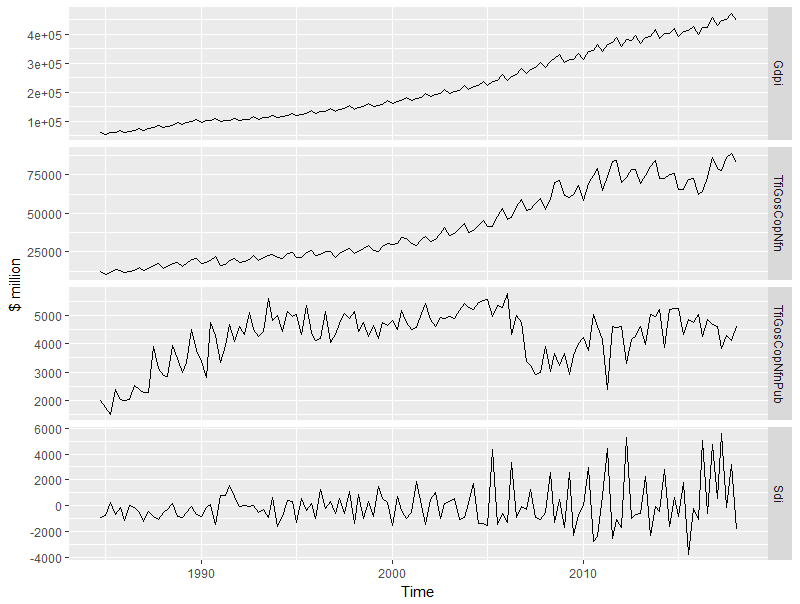
\includegraphics[scale=0.50]{Figs/TS-plots/INC-hierarchy/INC-char-of-levels-TSplots.png}
	\caption{Time plots for series from different levels of income hierarchy.}\label{TS-Inc}
\end{figure}

\begin{figure}[H]
	\centering
	\small
	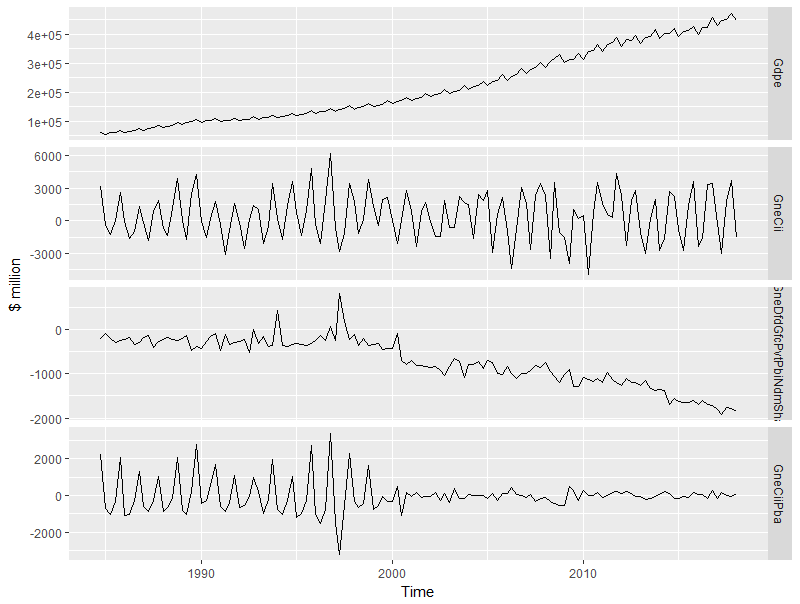
\includegraphics[scale=0.50]{Figs/TS-plots/EXP-hierarchy/EXP-char-of-levels-TSplots.png}
	\caption{Time plots for series from different levels of expenditure hierarchy.}\label{TS-Exp}
\end{figure}


\clearpage	


6. Experimental Design and
- setup: Time frame of Rolling window,
- alternative methods: ARIMA/base vs \naive, BU, OLS, WLS, MinT(Shrink).
- evaluation

- Point: MASE, MASE
- Probabilistic: CRPS, Energy Score
Skill score.

7. Results

\section{Methodology}\label{sec:meth}

We now demonstrate the potential for reconciliation methods to improve forecast accuracy for Australian GDP data.  We consider forecasts from $h=1$ quarter ahead forecasts up to $h=4$ quarter ahead using an {\em expanding} window.  First, the training sample is set to QX of XXXX to QX of XXXX and forecasts are produced for QX of XXXX to QX of XXXX. Then the training window is expanded one period ahead, i.e. from QX of XXXX to QX of XXXX with forecasts produces for QX of XXXX to QX of XXXX.  All up this leads to XX forecasts.

{\color{red} Need to get these dates off Puwasala.  Also last section may need to be changed}

\subsection{Models}

The first task in forecasting time series is to obtain base forecasts for all series in the hierarchy.  In the case of the income approach this necessitates forecasting XX time series while in the case of the expenditure approach forecasts for XX time series must be obtained.  As such our focus was on a methodology that was fast but flexible.  We consider simple univariate ARIMA models, where model order is selected via a combination of unit root testing and AIC using an algorithm developed by XXX and implement in the auto.arima function in XXX. {\color{red} Cite this to Rob's satisfaction}.  A similar approach was also undertaken using the ETS framework to produce base forecasts.  This had minimal impact on our conclusions with respect to forecast reconciliation methods, and in most cases ARIMA forecats outperformed ETS forecasts.  Consequently, results for ETS models are excluded but are available from the authors upon request {\color{red} again do we put this in an appendix?}.  We note that a number of more complicated approaches could have been used to obtain base forecasts including multivariate models such as vector autoregressions and models and methods that handle a large number of predictors such as factor models or least angle regresssion.  However, \cite{PanEtAl2019} show that univariate ARIMA models are highly competitive for forecasting Australian GDP even compared to these methods, and in any case our primary motivation is to demonstrate the potential of forecast reconciliation.

The forecast reconciliation approaches that we consider are bottom up, OLS, WLS with {\color{red} What scaling did we use} and the MinT (shrink) approach.  The MinT (sample) approach was also used but due to the size of the hierarchy forecasts reconciled via this approach were less stable.  Finally, all forecasts both base and reconciled are compared to a \naive benchmark.  Since the data are not deseasonalised, the \naive benchmark is a seasonal random walk, i.e. the forecast for GDP (or one of its components) is the realised GDP in the same quarter of the previous year.  The \naive forecast is by construction coherent and therefore does not need to be reconciled.

\subsection{Evaluation}

For evaluating point forecasts we consider two metrics, the Root Mean Squared Error (RMSE) and the Mean Absolute Scaled Error (MASE).  The absolute scaled error is defined as
\begin{equation*}
q_{t+h} = \sum \frac{|\breve{e}_{t+h|t}|}{(T-4)^{-1}\sum_{k=m+1}^{T}|y_k - y_{k-4}|}\,,
\end{equation*}
where $\breve{e}_{t+h}$\footnote{breve is used instead of a hat or tilde to denote that this can be the error either a base or reconciled forecast} is the difference between any forecast and the realisation {\color{red} 44444 check m is and change since m is bottom level dimension}.  An advantage of using MASE is that it is a scale independent measure. This is particularly relevant for hierarchical time series, since aggregate series by their very nature are on a larger scale than disaggregate series.  As such scale dependent metrics may unfairly favour methods that perform well for the aggregate series but poorly for disaggregate series.  For more details on different point forecast accuracy measures refer to \cite{hyndman2018forecasting}.

Forecast accuracy of probabilistic forecasts can be evaluated using scoring rules \cite{Gneiting2014}.  Let $\breve{F}$ be a probabilistic forecast and let $\breve{\vec{y}}\sim \breve{F}$  where breve is used to denote that either base forecast or reconciled forecast can be evaluated.  The accuracy of multivariate probabilistic forecasts will be measured by the energy score given by
\begin{equation*}
eS(\breve{F}_{T+h|T},\vec{y}_{T+h}) =
E_{\breve{F}}\|\breve{\vec{y}}_{T+h}-\vec{y}_{T+h}\|^\alpha
-\frac{1}{2}E_{\breve{F}}\|\breve{\vec{y}}_{T+h}-\breve{\vec{y}}^*_{T+h}\|^\alpha\,,
\end{equation*} where $\vec{y}_{T+h}$ is the realisation at time $T+h$, $\alpha\in (0,2]$. {\color{red} What did we use for alpha?}.  The expectations can be evaluated numerically as long as a sample from $\breve{F}$ is available which is the case for all methods we employ.  An advantage of using energy score is that in the univariate case it simplifies to the commonly used cumulative rank probability score (CRPS) given by

\begin{equation} \label{eq:24}
\text{CRPS}(\breve{F}_i,y_{i,T+h}) = E_{\breve{F}_i}|\breve{y}_{i,T+h}-y_{i,T+h}| - \frac{1}{2}E_{\breve{F}_i}|\breve{y}_{i,T+h}-\breve{y}^*_{i,T+h}|,
\end{equation}

where the subscript $i$ is used to denote that CRPS measures forecast accuracy for a single variable in the hierarchy.

As an alternative to the energy score, log score and variogram scores were also considered.  The log score was disregarded since \cite{Gamakumara2018} prove that the log score is improper with respect to the class of incoherent probabilistic forecasts when the true DGP is coherent.  The variogram score gave similar results to the energy score; variogram score results are omitted for brevity but are available from the authors upon request. {\color{red} or we put them in an appendix}


%\subsubsection{Comparison between different forecasting methods}
%
%{\color{red}To be included in results section - and discussed much more briefly.}
%
%We are mainly interested to evaluate the hierarchical forecasts in two aspects. One is to examine whether the having coherent forecasts is improving the forecast accuracy. This can be evaluated by comparing the incoherent forecasts with any coherent forecasts in both point as well as probabilistic framework. Secondly we are interested in finding the best reconciliation method by comparing reconciled forecast from different reconciliation methods.
%
%For any comparison we use Skill score as defined in \citep{Gneiting2007}. For a given forecasting method, evaluated by a particular scoring rule $S(\cdot)$ , the skill score can be calculated as follows,
%\begin{equation} \label{eq:25}
%Ss[S_B(\cdot)] = \frac{S_B(\bm{Y},\bm{y})^{\text{ref}} - S_B(\breve{\bm{Y}},\bm{y})}{S_B(\bm{Y},\bm{y})^{\text{ref}}}\times 100\%,
%\end{equation}
%where $S_B(\cdot)$ is average score over $B$ replicates and $S_B(\bm{Y},\bm{y})^{\text{ref}}$ is the average score of the reference forecasting methods. Thus $Ss[S_B(\cdot)]$ gives the percentage improvement of the preferred forecasting method relative to the reference method. Any positive value indicates that method is superior to the reference method, whereas any negative value of $Ss[S_B(\cdot)]$ indicate that the method we compared is poor than the reference method.
%
%
%
%
%First step in the reconciliation process is to generate base forecasts in both point and probabilistic frameworks. Thus we fit ETS and ARIMA models for each individual series of the hierarchy by using default settings in forecast package in R software implemented by \citep{Hyndman2018}. We further use seasonal naive forecasts as the benchmark which are always coherent.



\textcolor{red}{Discuss results}

\begin{figure}[H]
	\centering
	\small
	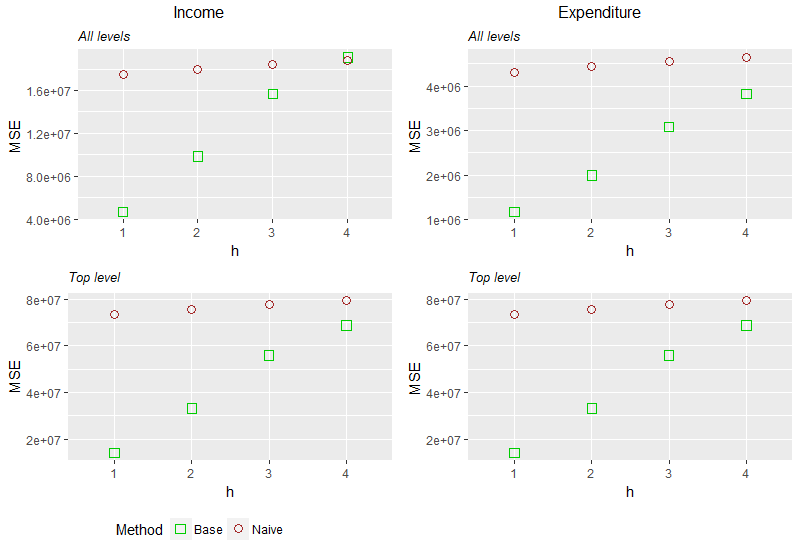
\includegraphics[scale=0.50]{Figs/Results/NaiveVsBase_MSE.png}
	\caption{Skill scores for naive forecasts based on MSE}\label{NaiveVsBase_MSE}
\end{figure}

\begin{figure}[H]
	\centering
	\small
	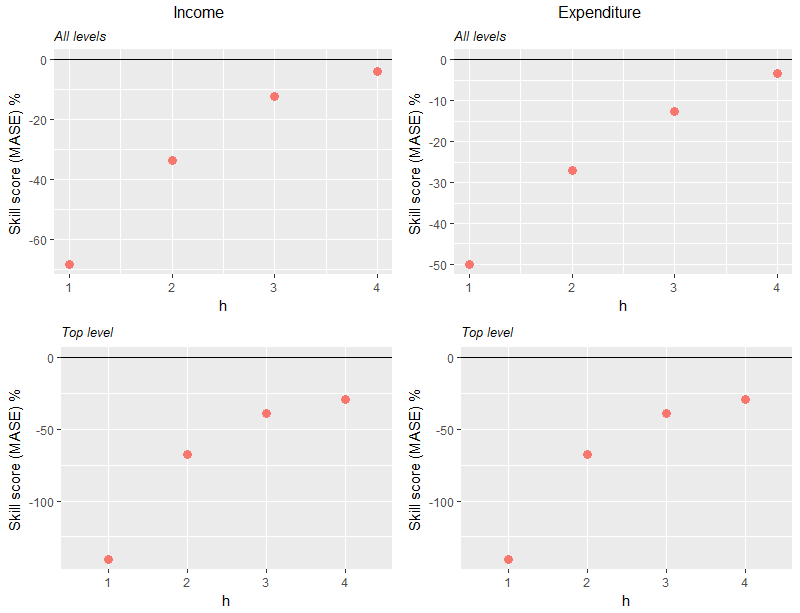
\includegraphics[scale=0.50]{Figs/Results/NaiveVsBase_MASE.png}
	\caption{Skill scores for naive forecasts based on MASE}\label{NaiveVsBase_MASE}
\end{figure}
\subsubsection*{Income approach}

\begin{figure}[H]
	\centering
	\small
	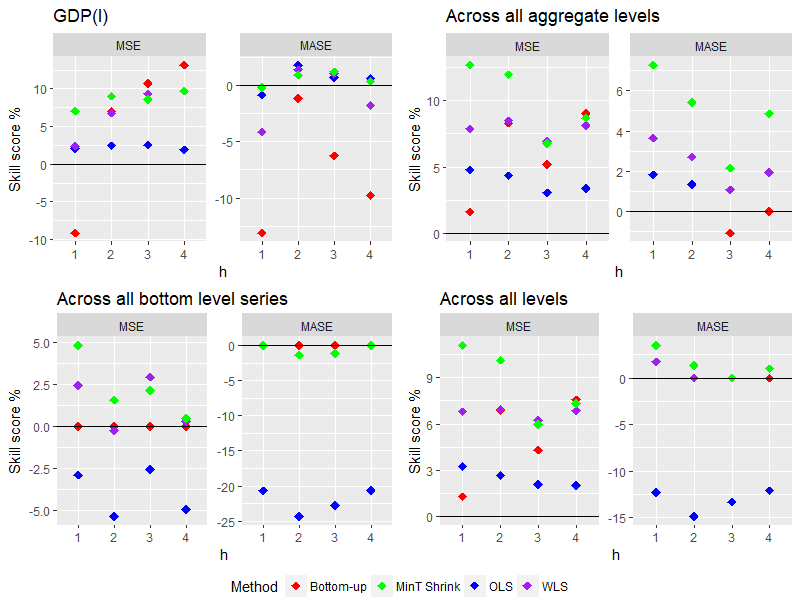
\includegraphics[scale=0.50]{Figs/Results/INC-PointF.png}
	\caption{Summary of point forecasts in income approach}\label{Exp-PointF}
\end{figure}


\subsubsection*{Expenditure approach}

\begin{figure}[H]
	\centering
	\small
	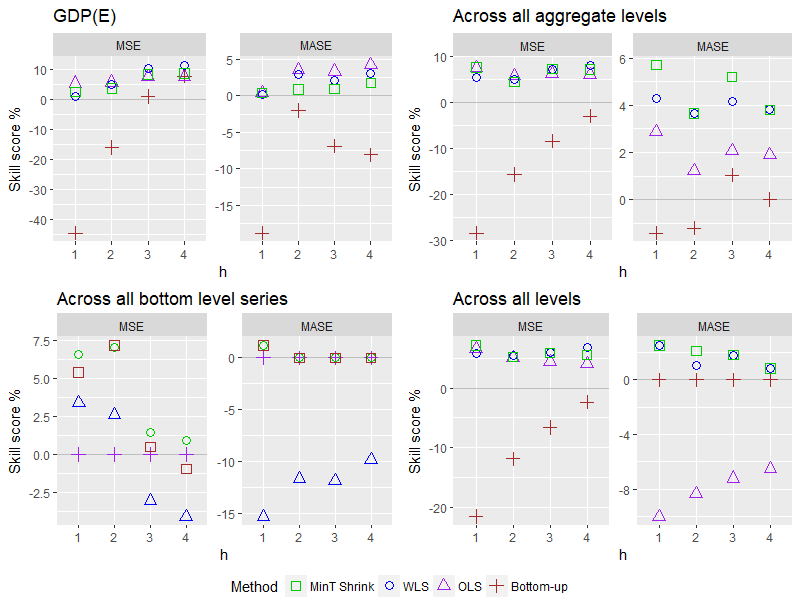
\includegraphics[scale=0.50]{Figs/Results/EXP-PointF.png}
	\caption{Summary of point forecasts in expenditure approach}\label{Inc-PointF}
\end{figure}




\section{Results}\label{sec:results}

Results are presented in \ref{Tab: Inc_PointF} and \ref{Tab: Exp_PointF} for income and expenditure approaches respectively. \\

Results are presented in tables \ref{Tab: Inc_ProbGaus_ES_VS}, \ref{Tab: Inc_ProbGaus_LS}, \ref{Tab: Inc_ProbGaus_UnivS} for income approach and \ref{Tab: Exp_ProbGaus_ES_VS}, \ref{Tab: Exp_ProbGaus_LS}, \ref{Tab: Exp_ProbGaus_UnivS} for expenditure approach. \\

\textcolor{red}{Discuss results}


\textcolor{red}{Possible discuss skill scores}

\textcolor{red}{Discuss breakdown into looking at different levels.}

\subsection*{Income approach}

\begin{figure}[H]
	\centering
	\small
	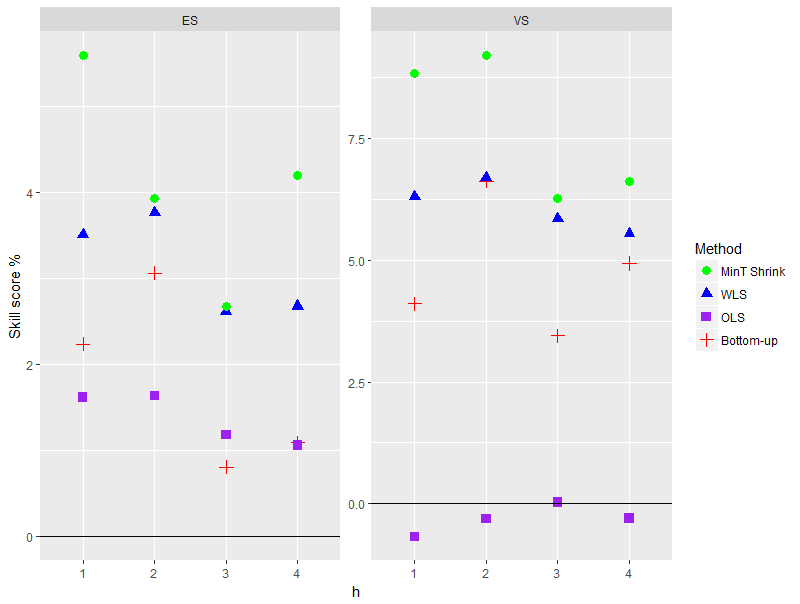
\includegraphics[scale=0.50]{Figs/Results/INC-ProbGaussF-MultivS_ES_VS.png}
	\caption{Skill scores with respect to energy score and variogram score for multivariate Gaussian forecast distribution of income hierarchy}\label{Inc_ProbGaus_ES_VS}
\end{figure}

\begin{figure}[H]
	\centering
	\small
	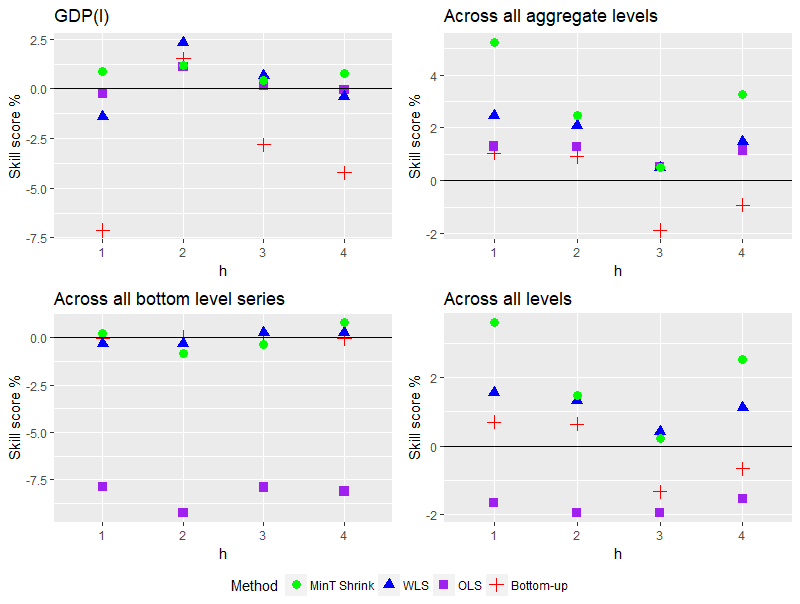
\includegraphics[scale=0.50]{Figs/Results/INC-ProbGaussF-UnivS_CRPS.png}
	\caption{Skill scores for univariate Gaussian forecast distributions of individual series of income hierarchy}\label{Inc_ProbGaus_UnivS}
\end{figure}


\subsection*{Expenditure approach}

\begin{figure}[H]
	\centering
	\small
	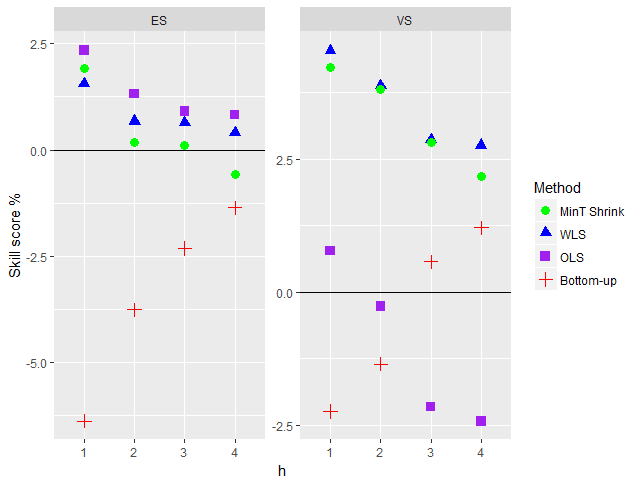
\includegraphics[scale=0.50]{Figs/Results/EXP-ProbGaussF-MultivS_ES_VS.png}
	\caption{Skill scores with respect to energy score and variogram score for multivariate Gaussian forecast distribution of expenditure hierarchy}\label{Exp_ProbGaus_ES_VS}
\end{figure}

\begin{figure}[H]
	\centering
	\small
	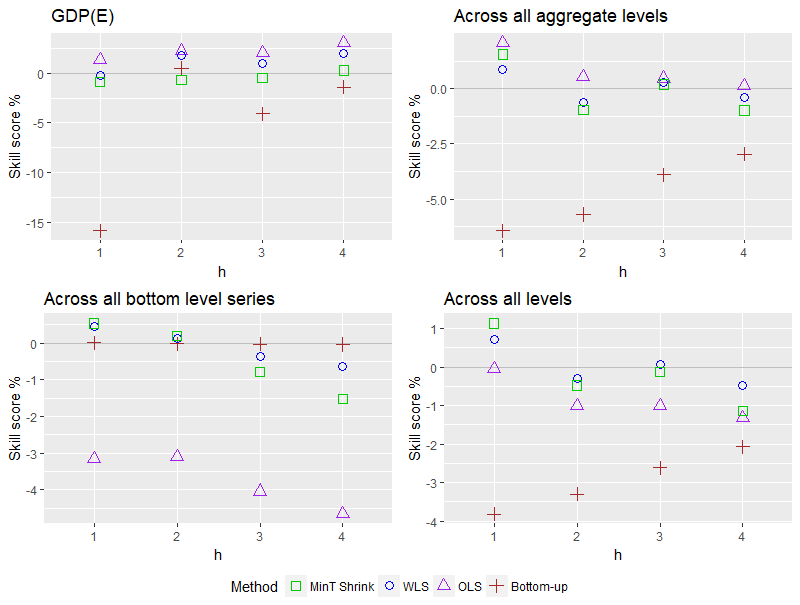
\includegraphics[scale=0.50]{Figs/Results/EXP-ProbGaussF-UnivS_CRPS.png}
	\caption{Skill scores for univariate Gaussian forecast distributions of individual series of expenditure hierarchy}\label{Exp_ProbGaus_UnivS}
\end{figure}










\subsubsection{Non-parametric probabilistic forecasts for Australian GDP}

We also estimate the coherent probabilistic forecasts for GDP and its disaggregate components by using the non-parametric bootstrap approach explained in the section (?).

\subsection*{Income approach}

\begin{figure}[H]
	\centering
	\small
	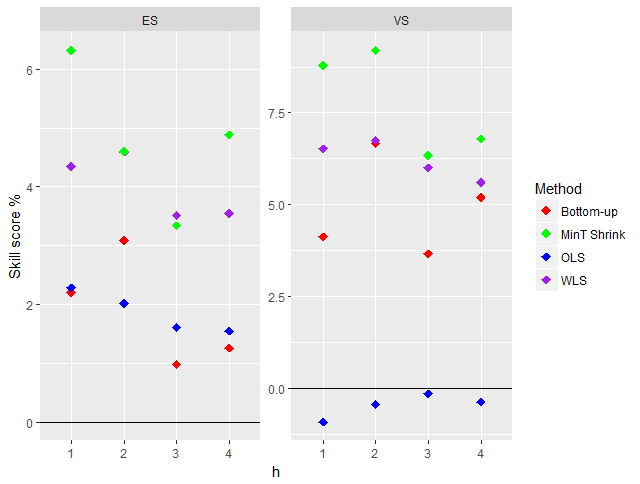
\includegraphics[scale=0.50]{Figs/Results/INC-ProbNonParaF-MultivS_ES_VS.png}
	\caption{Skill scores with respect to energy score and variogram score for multivariate Gaussian forecast distribution of income hierarchy}\label{Inc_ProbNonParF_ES_VS}
\end{figure}

\begin{figure}[H]
	\centering
	\small
	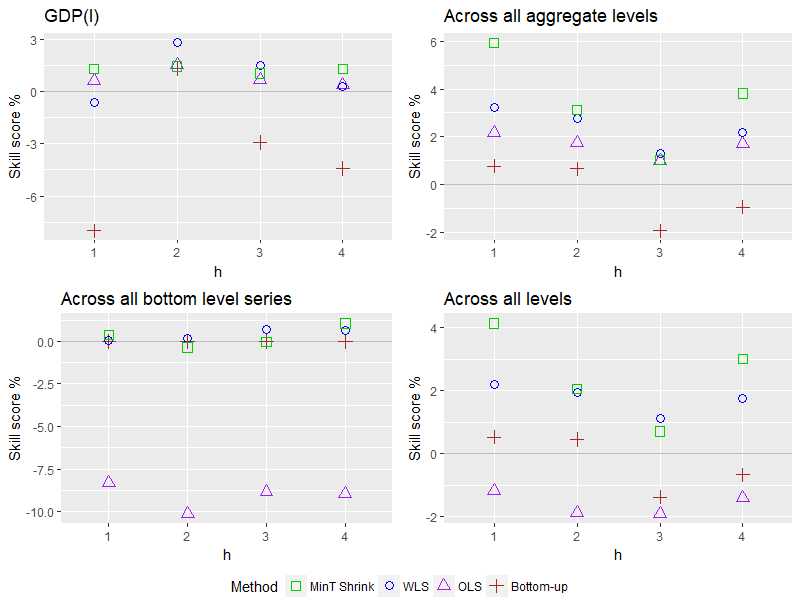
\includegraphics[scale=0.50]{Figs/Results/INC-ProbNonParaF-UnivS_CRPS.png}
	\caption{Skill scores for univariate Gaussian forecast distributions of individual series of income hierarchy}\label{Inc_ProbNonParF_UnivS}
\end{figure}






\subsection*{Expenditure approach}

\begin{figure}[H]
	\centering
	\small
	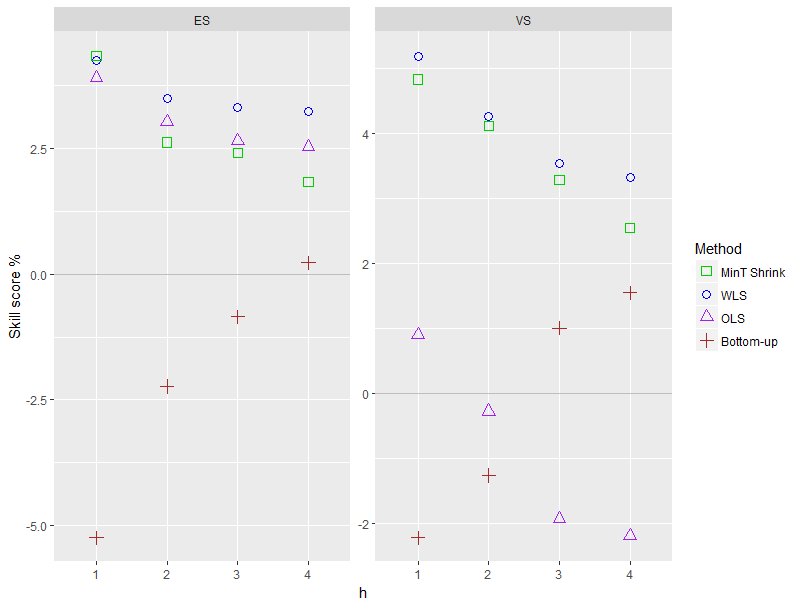
\includegraphics[scale=0.50]{Figs/Results/EXP-ProbNonParaF-MultivS_ES_VS.png}
	\caption{Skill scores with respect to energy score and variogram score for multivariate Gaussian forecast distribution of expenditure hierarchy}\label{Exp_ProbNonParF_ES_VS}
\end{figure}

\begin{figure}[H]
	\centering
	\small
	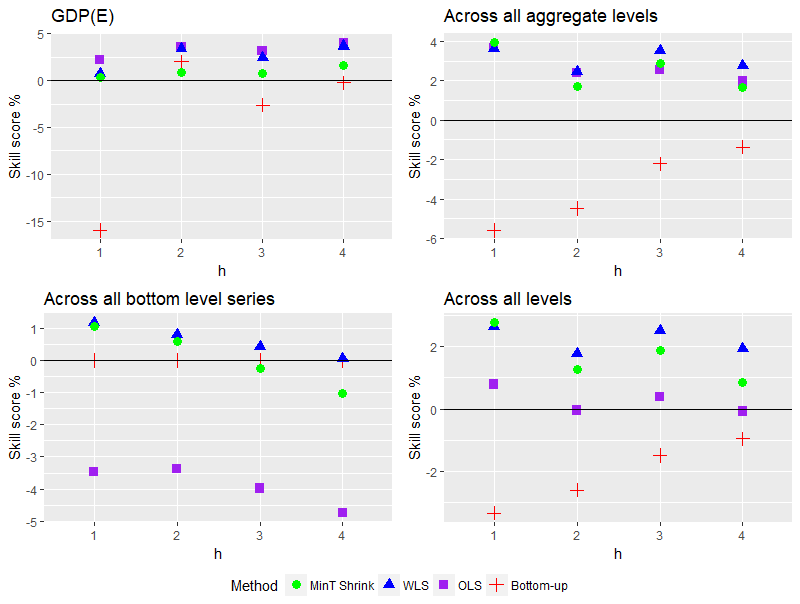
\includegraphics[scale=0.50]{Figs/Results/EXP-ProbNonParaF-UnivS_CRPS.png}
	\caption{Skill scores for univariate Gaussian forecast distributions of individual series of expenditure hierarchy}\label{Exp_ProbNonParF_UnivS}
\end{figure}




\pagebreak



\section*{Appendix}
\addcontentsline{toc}{section}{Appendix 1}

\begin{figure}[H]
	\centering
	\small
	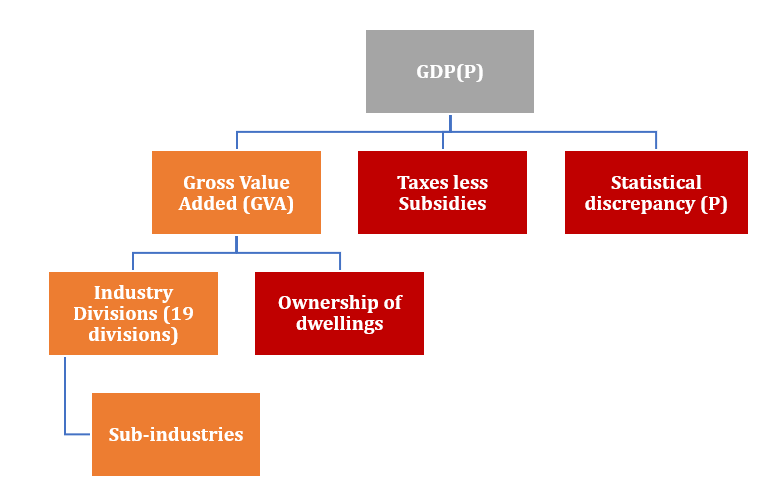
\includegraphics[scale=0.65]{Figs/GDP_P_fig1.PNG}
	\caption{Hierarchy of production approach.}\label{GDP_P_fig1}
\end{figure}

\begin{figure}[H]
	\centering
	\small
	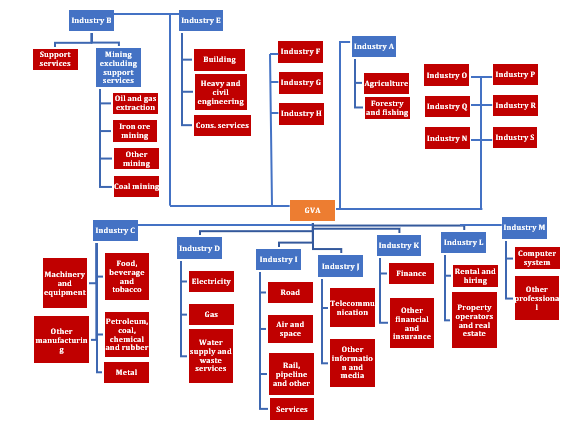
\includegraphics[scale=0.65]{Figs/GDP_P_fig2.PNG}
	\caption{Hierarchy of GVA under production approach.}\label{GDP_P_fig2}
\end{figure}

\begin{figure}[H]
	\centering
	\small
	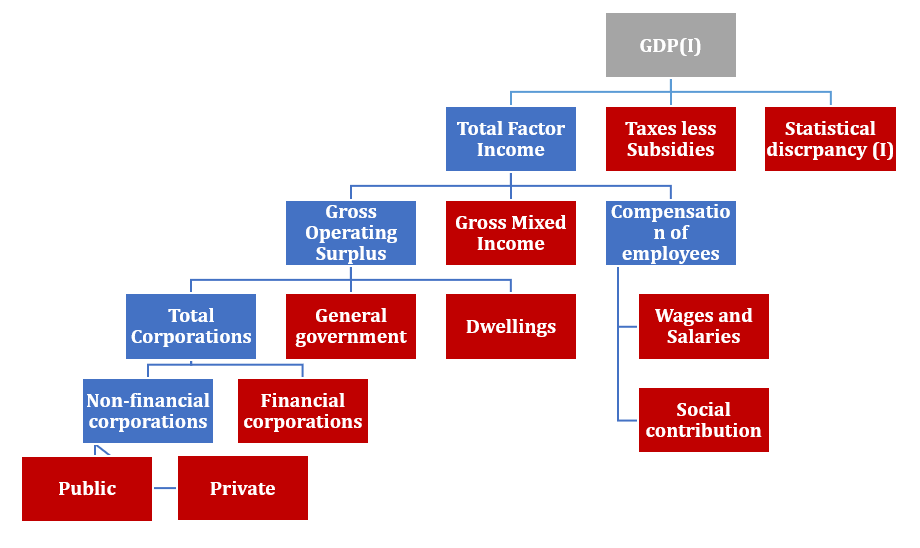
\includegraphics[scale=0.65]{Figs/GDP_I_fig1.PNG}
	\caption{Hierarchy of income approach.}\label{GDP_I_fig1}
\end{figure}

\begin{align*}
GDP(E) &= \textit{Final consumption expenditure} + \textit{Gross fixed capital formation} + \textit{Changes in inventories} +\\ &\textit{Exports of goods and services} - \textit{Imports of goods and services} + \textit{Statistical decrepency (E)}\\
\end{align*}
Associated hierarchical structure is given in figure \ref{GDP_E_fig1}, \ref{GDP_E_fig2} and \ref{GDP_E_fig3}.

\begin{figure}[H]
	\centering
	\small
	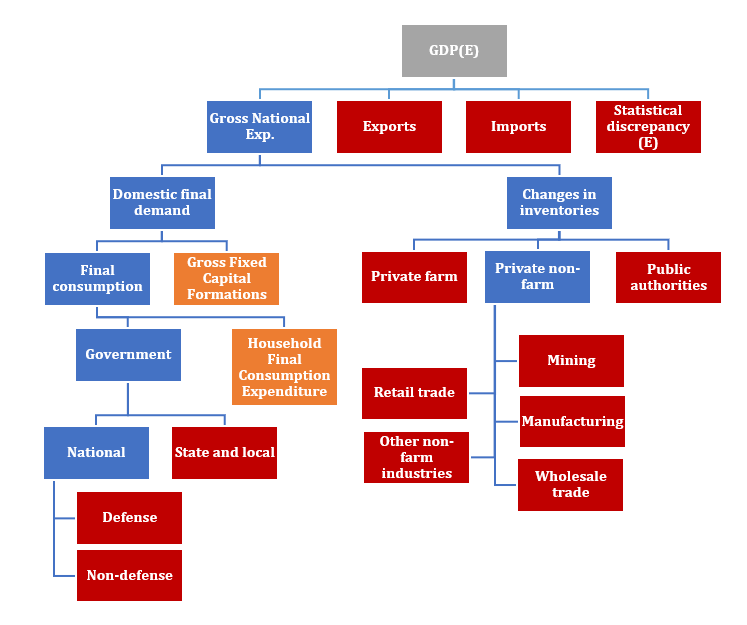
\includegraphics[scale=0.65]{Figs/GDP_E_fig1.PNG}
	\caption{Hierarchy of expenditure approach.}\label{GDP_E_fig1}
\end{figure}

\begin{figure}[H]
	\centering
	\small
	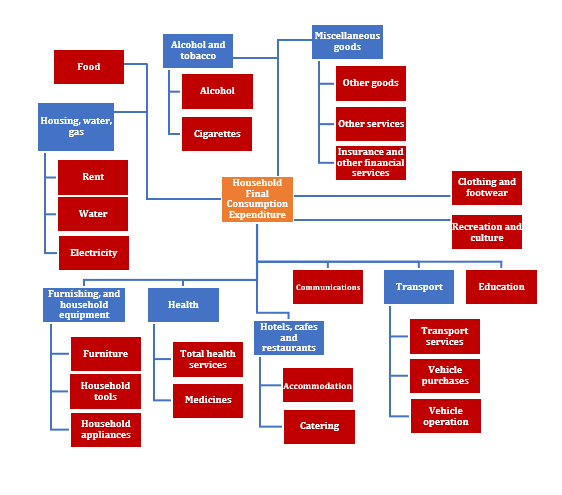
\includegraphics[scale=1]{Figs/GDP_E_fig2.PNG}
	\caption{Household final consumption expenditure under expenditure approach.}\label{GDP_E_fig2}
\end{figure}

\begin{figure}[H]
	\centering
	\small
	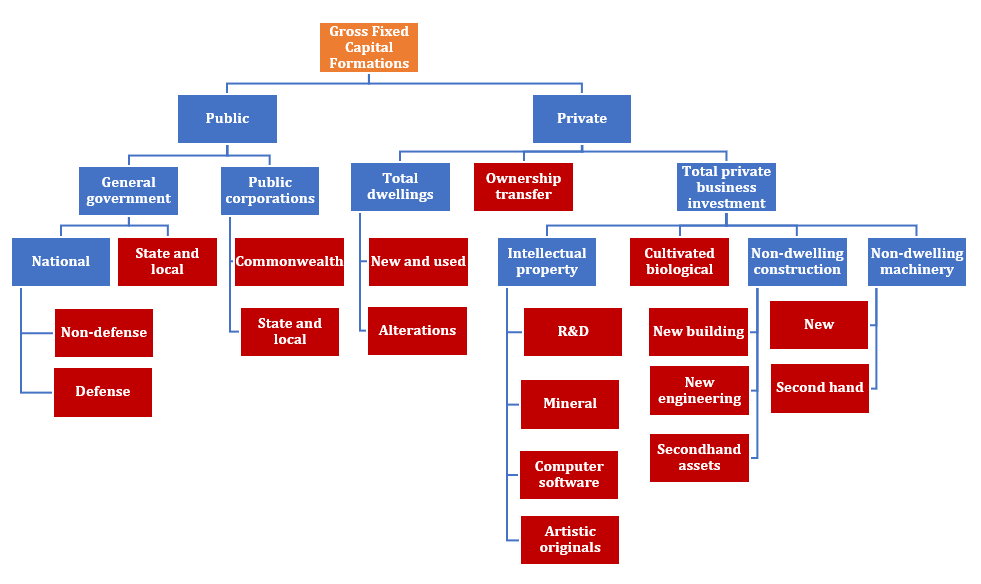
\includegraphics[scale=0.65]{Figs/GDP_E_fig3.PNG}
	\caption{Gross fixed capital formation (GFCF) under expenditure approach.}\label{GDP_E_fig3}
\end{figure}


\begin{table}[H]
	\caption{Variables, Series IDs and their descriptions for Income Approach}
	\centering
	\resizebox{\linewidth}{!}{
		\begin{tabular}[t]{lll}
			\toprule
			\textbf{Variable} & \textbf{Series ID} & \textbf{Description}\\
			\midrule
			Gdpi & A2302467A & GDP(I)\\
			Sdi & A2302413V & Statistical discrepancy (I)\\
			Tsi & A2302412T & Taxes less subsidies (I)\\
			TfiCoeWns & A2302399K & Compensation of employees; Wages and salaries\\
			TfiCoeEsc & A2302400J & Compensation of employees; Employers' social contributions\\
			\addlinespace
			TfiCoe & A2302401K & Compensation of employees\\
			TfiGosCopNfnPvt & A2323369L & Private non-financial corporations; Gross operating surplus\\
			TfiGosCopNfnPub & A2302403R & Public non-financial corporations; Gross operating surplus\\
			TfiGosCopNfn & A2302404T & Non-financial corporations; Gross operating surplus\\
			TfiGosCopFin & A2302405V & Financial corporations;  Gross operating surplus\\
			\addlinespace
			TfiGosCop & A2302406W & Total corporations; Gross operating surplus\\
			TfiGosGvt & A2298711F & General government; Gross operating surplus\\
			TfiGosDwl & A2302408A & Dwellings owned by persons; Gross operating surplus\\
			TfiGos & A2302409C & All sectors; Gross operating surplus\\
			TfiGmi & A2302410L & Gross mixed income\\
			Tfi & A2302411R & Total factor income\\
			\bottomrule
		\end{tabular}
		\label{Tab: Income-hierarchy}
	}
\end{table}

\begin{table}[H]
	\caption{Variables, Series IDs and their descriptions for Expenditure Approach}
	\centering
	\resizebox{\linewidth}{!}{
		\begin{tabular}[t]{lll}
			\toprule
			\textbf{Variable} & \textbf{Series ID} & \textbf{Description}\\
			\midrule
			
			Gdpe & A2302467A & GDP(E)\\
			Sde & A2302566J & Statistical Discrepancy(E)\\
			Exp & A2302564C & Exports of goods and services\\
			Imp & A2302565F & Imports of goods and services\\
			Gne & A2302563A & Gross national exp.\\
			\addlinespace
			GneDfdFceGvtNatDef & A2302523J & Gen. gov. - National; Final consumption exp. - Defence\\
			GneDfdFceGvtNatNdf & A2302524K & Gen. gov. - National; Final consumption exp. - Non-defence\\
			GneDfdFceGvtNat & A2302525L & Gen. gov. - National; Final consumption exp.\\
			GneDfdFceGvtSnl & A2302526R & Gen. gov. - State and local; Final consumption exp,\\
			GneDfdFceGvt & A2302527T & Gen. gov.; Final consumption exp.\\
			\addlinespace
			GneDfdFce & A2302529W & All sectors; Final consumption exp.\\
			GneDfdGfcPvtTdwNnu & A2302543T & Pvt.; Gross fixed capital formation (GFCF)\\
			GneDfdGfcPvtTdwAna & A2302544V & Pvt.; GFCF - Dwellings - Alterations and additions\\
			GneDfdGfcPvtTdw & A2302545W & Pvt.; GFCF - Dwellings - Total\\
			GneDfdGfcPvtOtc & A2302546X & Pvt.; GFCF - Ownership transfer costs\\
			\addlinespace
			GneDfdGfcPvtPbiNdcNbd & A2302533L & Pvt. GFCF - Non-dwelling construction - New building\\
			GneDfdGfcPvtPbiNdcNec & A2302534R & Pvt.; GFCF - Non-dwelling construction -\\
			&  & New engineering construction\\
			GneDfdGfcPvtPbiNdcSha & A2302535T & Pvt.; GFCF - Non-dwelling construction -\\
			&  & Net purchase of second hand \vphantom{1} assets\\
			\addlinespace
			GneDfdGfcPvtPbiNdc & A2302536V & Pvt.; GFCF - Non-dwelling construction - Total\\
			GneDfdGfcPvtPbiNdmNew & A2302530F & Pvt.; GFCF - Machinery and equipment - New\\
			GneDfdGfcPvtPbiNdmSha & A2302531J & Pvt.; GFCF - Machinery and equipment -\\
			&  & Net purchase of second hand assets\\
			GneDfdGfcPvtPbiNdm & A2302532K & Pvt.; GFCF - Machinery and equipment - Total\\
			\addlinespace
			GneDfdGfcPvtPbiCbr & A2716219R & Pvt.; GFCF - Cultivated biological resources\\
			GneDfdGfcPvtPbiIprRnd & A2716221A & Pvt.; GFCF - Intellectual property products -\\
			&  & Research and development\\
			GneDfdGfcPvtPbiIprMnp & A2302539A & Pvt.; GFCF - Intellectual property products -\\
			&  & Mineral and petroleum exploration\\
			\addlinespace
			GneDfdGfcPvtPbiIprCom & A2302538X & Pvt.; GFCF - Intellectual property products - Computer software\\
			GneDfdGfcPvtPbiIprArt & A2302540K & Pvt.; GFCF - Intellectual property products - Artistic originals\\
			GneDfdGfcPvtPbiIpr & A2716220X & Pvt.; GFCF - Intellectual property products Total\\
			GneDfdGfcPvtPbi & A2302542R & Pvt.;  GFCF - Total private business investment\\
			GneDfdGfcPvt & A2302547A & Pvt.; GFCF\\
			\addlinespace
			GneDfdGfcPubPcpCmw & A2302548C & Plc. corporations - Commonwealth; GFCF\\
			GneDfdGfcPubPcpSnl & A2302549F & Plc. corporations - State and local; GFCF\\
			GneDfdGfcPubPcp & A2302550R & Plc. corporations; GFCF Total\\
			GneDfdGfcPubGvtNatDef & A2302551T & Gen. gov. - National; GFCF - Defence\\
			GneDfdGfcPubGvtNatNdf & A2302552V & Gen. gov. - National ; GFCF - Non-defence\\
			\addlinespace
			GneDfdGfcPubGvtNat & A2302553W & Gen. gov. - National ; GFCF Total\\
			GneDfdGfcPubGvtSnl & A2302554X & Gen. gov. - State and local; GFCF\\
			GneDfdGfcPubGvt & A2302555A & Gen. gov.; GFCF\\
			GneDfdGfcPub & A2302556C & Plc.; GFCF\\
			GneDfdGfc & A2302557F & All sectors; GFCF\\
			\bottomrule
		\end{tabular}
		
		\label{Tab:Expenditure-hierarchy-1}
	}
\end{table}

\begin{table}[H]
	\caption{Variables, Series IDs and their descriptions for Changes in Inventories - Expenditure Approach}
	\centering
	\resizebox{\linewidth}{!}{
		\begin{tabular}[t]{lll}
			
			\toprule
			\textbf{Variable} & \textbf{Series ID} & \textbf{Description}\\
			\midrule
			
			GneCii & A2302562X & Changes in Inventories\\
			GneCiiPfm & A2302560V & Farm\\
			GneCiiPba & A2302561W & Public authorities\\
			GneCiiPnf & A2302559K & Private; Non-farm Total\\
			GneCiiPnfMin & A83722619L & Private; Mining (B)\\
			\addlinespace
			GneCiiPnfMan & A3348511X & Private; Manufacturing (C)\\
			GneCiiPnfWht & A3348512A & Private; Wholesale trade (F)\\
			GneCiiPnfRet & A3348513C & Private; Retail trade (G)\\
			GneCiiPnfOnf & A2302273C & Private; Non-farm; Other non-farm industries\\
			\bottomrule
		\end{tabular}
		\label{Tab:Expenditure-hierarchy-2}
	}
\end{table}

\begin{table}[H]
	\caption{Variables, Series IDs and their descriptions for Household Final Consumption - Expenditure Approach}
	\centering
	\resizebox{\linewidth}{!}{
		\begin{tabular}[t]{lll}
			
			\toprule
			\textbf{Variable} & \textbf{Series ID} & \textbf{Description}\\
			\midrule
			
			GneDfdHfc & A2302254W & Household Final Consumption Expenditure\\
			GneDfdFceHfcFud & A2302237V & Food\\
			GneDfdFceHfcAbt & A3605816F & Alcoholic beverages and tobacco\\
			GneDfdFceHfcAbtCig & A2302238W & Cigarettes and tobacco\\
			GneDfdFceHfcAbtAlc & A2302239X & Alcoholic beverages\\
			\addlinespace
			GneDfdFceHfcCnf & A2302240J & Clothing and footwear\\
			GneDfdFceHfcHwe & A3605680F & Housing, water, electricity, gas and other fuels\\
			GneDfdFceHfcHweRnt & A3605681J & Actual and imputed rent for housing\\
			GneDfdFceHfcHweWsc & A3605682K & Water and sewerage charges\\
			GneDfdFceHfcHweEgf & A2302242L & Electricity, gas and other fuel\\
			\addlinespace
			GneDfdFceHfcFhe & A2302243R & Furnishings and household equipment\\
			GneDfdFceHfcFheFnt & A3605683L & Furniture, floor coverings and household goods\\
			GneDfdFceHfcFheApp & A3605684R & Household appliances\\
			GneDfdFceHfcFheTls & A3605685T & Household tools\\
			GneDfdFceHfcHlt & A2302244T & Health\\
			\addlinespace
			GneDfdFceHfcHltMed & A3605686V & Medicines, medical aids and therapeutic appliances\\
			GneDfdFceHfcHltHsv & A3605687W & Total health services\\
			GneDfdFceHfcTpt & A3605688X & Transport\\
			GneDfdFceHfcTptPvh & A2302245V & Purchase of vehicles\\
			GneDfdFceHfcTptOvh & A2302246W & Operation of vehicles\\
			\addlinespace
			GneDfdFceHfcTptTsv & A2302247X & Transport services\\
			GneDfdFceHfcCom & A2302248A & Communications\\
			GneDfdFceHfcRnc & A2302249C & Recreation and culture\\
			GneDfdFceHfcEdc & A2302250L & Education services\\
			GneDfdFceHfcHcr & A2302251R & Hotels, cafes and restaurants\\
			\addlinespace
			GneDfdFceHfcHcrCsv & A3605694V & Catering services\\
			GneDfdFceHfcHcrAsv & A3605695W & Accommodation services\\
			GneDfdFceHfcMis & A3605696X & Miscellaneous goods and services\\
			GneDfdFceHfcMisOgd & A3605697A & Other goods\\
			GneDfdFceHfcMisIfs & A2302252T & Insurance and other financial services\\
			GneDfdFceHfcMisOsv & A3606485T & Other services\\
			\bottomrule
		\end{tabular}
		\label{Tab:Expenditure-hierarchy-3}
	}
\end{table}

\begin{figure}[H]
	\centering
	\small
	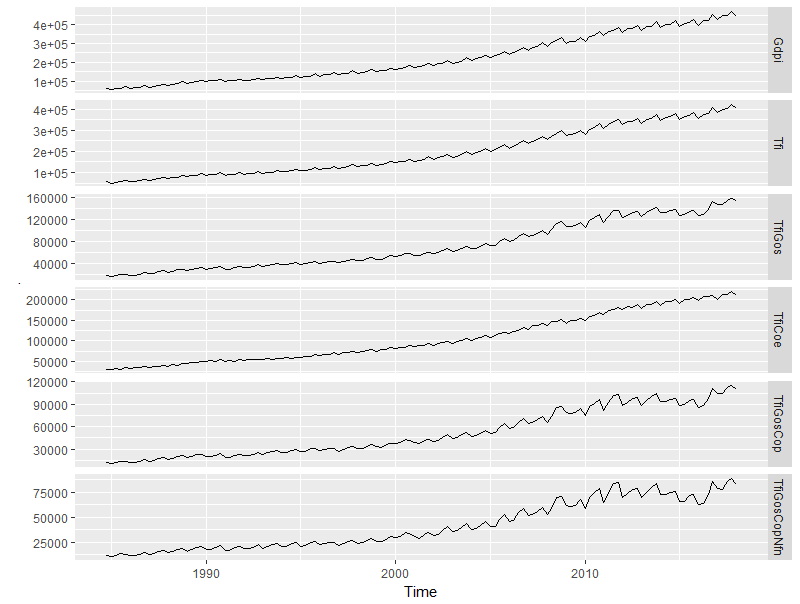
\includegraphics[scale=0.5]{Figs/TS-plots/INC-hierarchy/INC-aggregates_TSplots.png}
	\caption{All aggregate level series of income hierarchy.}\label{INC-aggregates_TSplot}
\end{figure}

\begin{figure}[H]
	\centering
	\small
	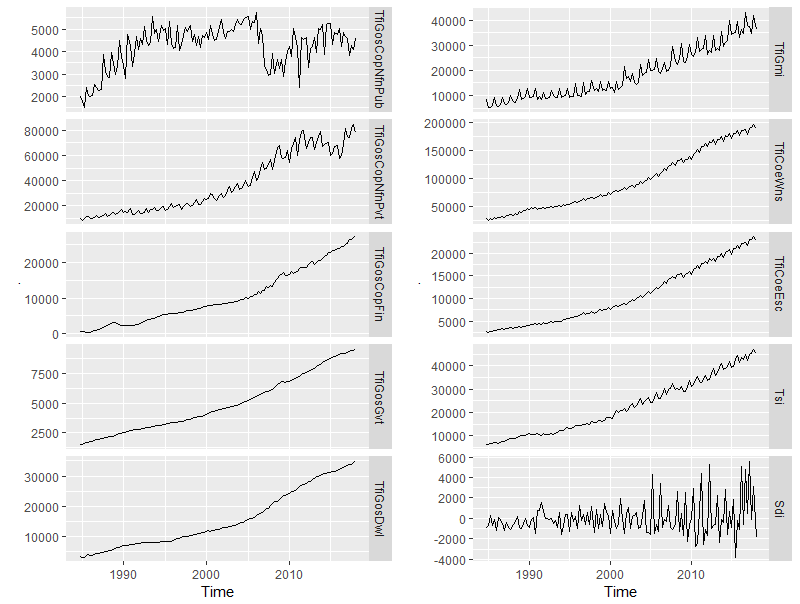
\includegraphics[scale=0.5]{Figs/TS-plots/INC-hierarchy/INC-bottomlevel-TSplots.png}
	\caption{All bottom level series of income hierarchy.}\label{INC-bottomlevel_TSplot}
\end{figure}

\begin{figure}[H]
	\centering
	\small
	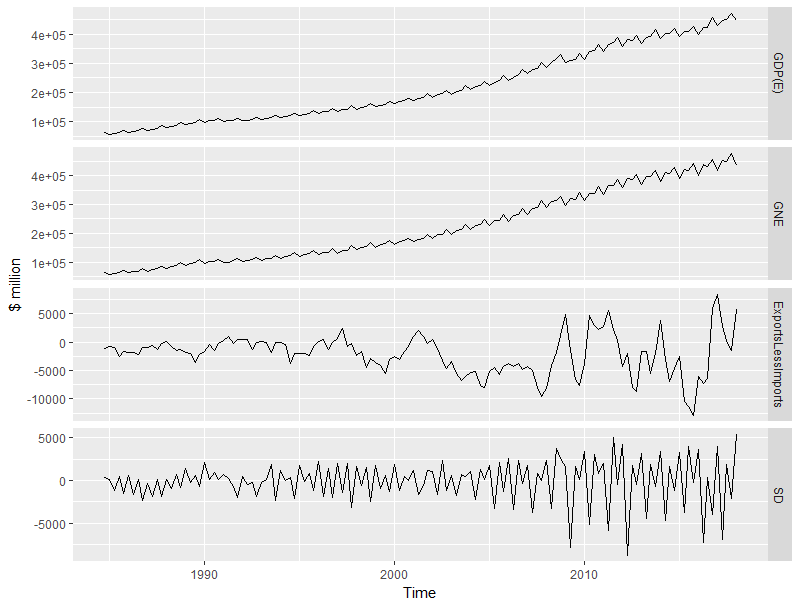
\includegraphics[scale=0.5]{Figs/TS-plots/EXP-hierarchy/set-1.png}
	\caption{GDP(E), GNE, Experts less Imports and Statistical discrepancy in expenditure hierarchy.}\label{EXP-set-1}
\end{figure}

\begin{figure}[H]
	\centering
	\small
	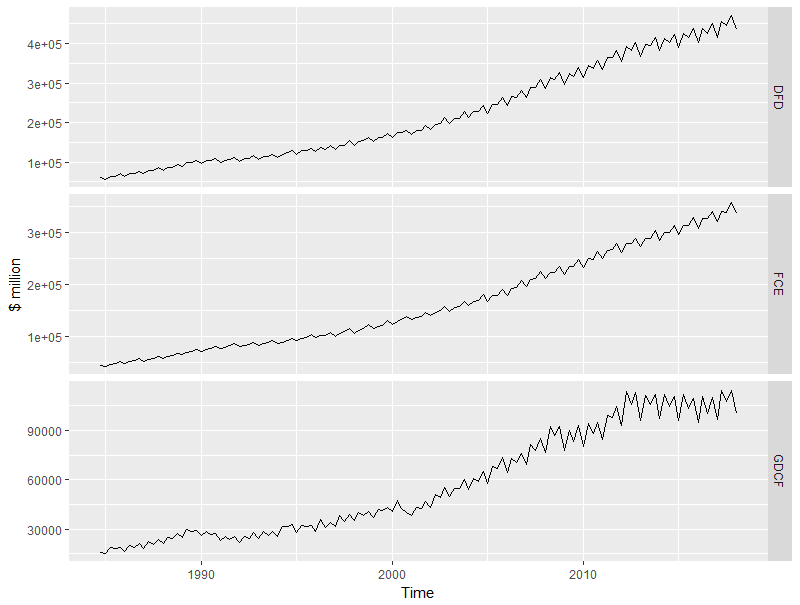
\includegraphics[scale=0.5]{Figs/TS-plots/EXP-hierarchy/set-2.png}
	\caption{Domestic Final Demand, Final Consumption Expenditure and Gross Fixed Capital Formations in expenditure hierarchy.}\label{EXP-set-2}
\end{figure}

\begin{figure}[H]
	\centering
	\small
	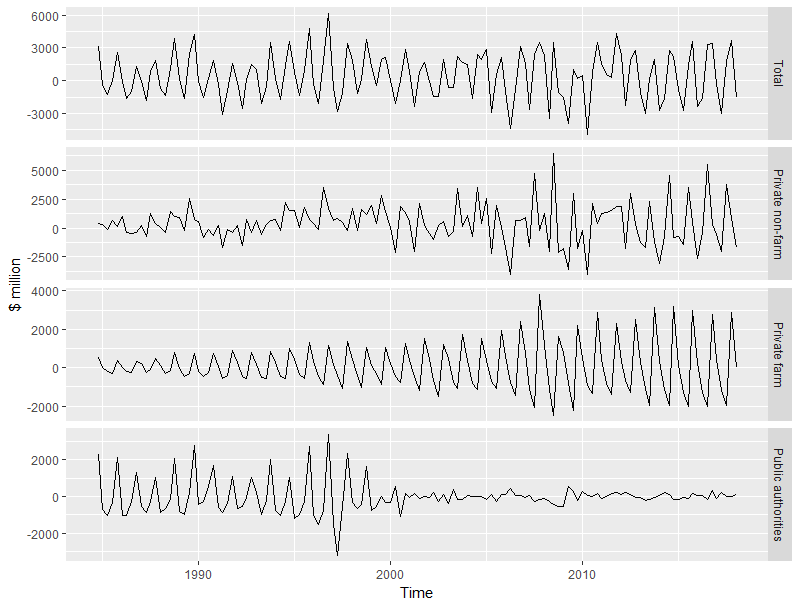
\includegraphics[scale=0.5]{Figs/TS-plots/EXP-hierarchy/set-3.png}
	\caption{Total changes in inventory, Private non-farm, Private farm and Public authorities in expenditure hierarchy.}\label{EXP-set-3}
\end{figure}

\begin{figure}[H]
	\centering
	\small
	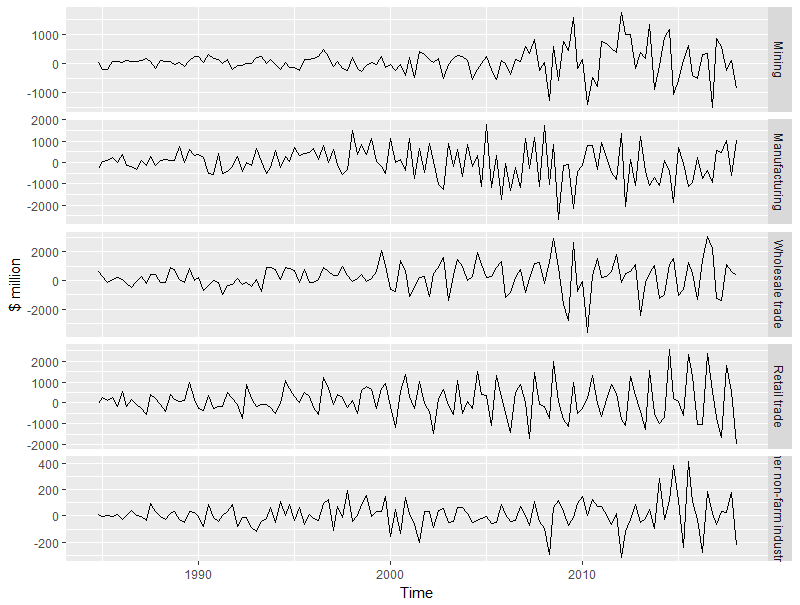
\includegraphics[scale=0.5]{Figs/TS-plots/EXP-hierarchy/set-4.png}
	\caption{Disaggregation of private non-farm in expenditure hierarchy.}\label{EXP-set-4}
\end{figure}

\begin{figure}[H]
	\centering
	\small
	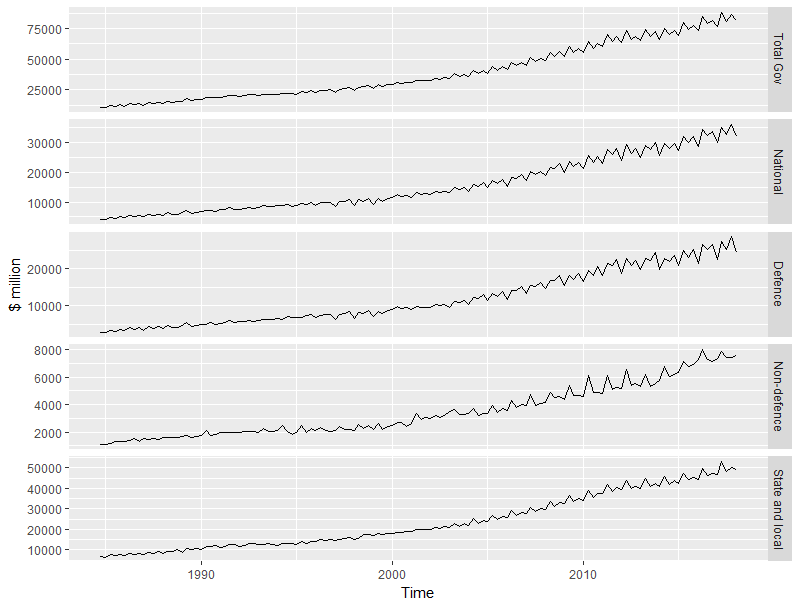
\includegraphics[scale=0.5]{Figs/TS-plots/EXP-hierarchy/set-5.png}
	\caption{Disaggregation of government final consumption expenditure.}\label{EXP-set-5}
\end{figure}

\begin{figure}[H]
	\centering
	\small
	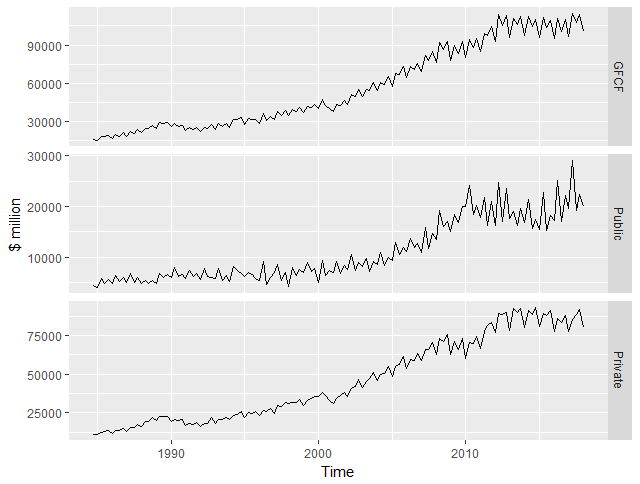
\includegraphics[scale=0.65]{Figs/TS-plots/EXP-hierarchy/set-6.png}
	\caption{Public, private and total fixed capital formations.}\label{EXP-set-6}
\end{figure}

\begin{figure}[H]
	\centering
	\small
	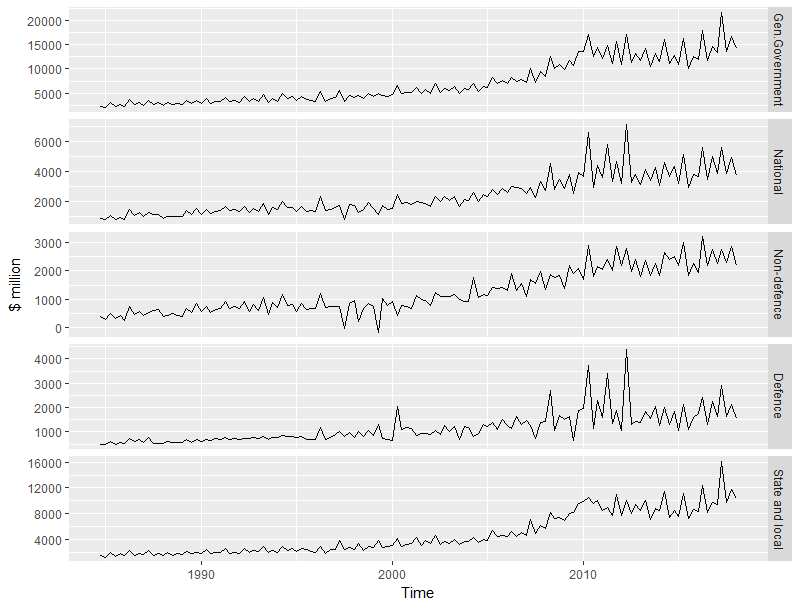
\includegraphics[scale=0.5]{Figs/TS-plots/EXP-hierarchy/set-7.png}
	\caption{Disaggregation of general government of Gross fixed capital formations.}\label{EXP-set-7}
\end{figure}

\begin{figure}[H]
	\centering
	\small
	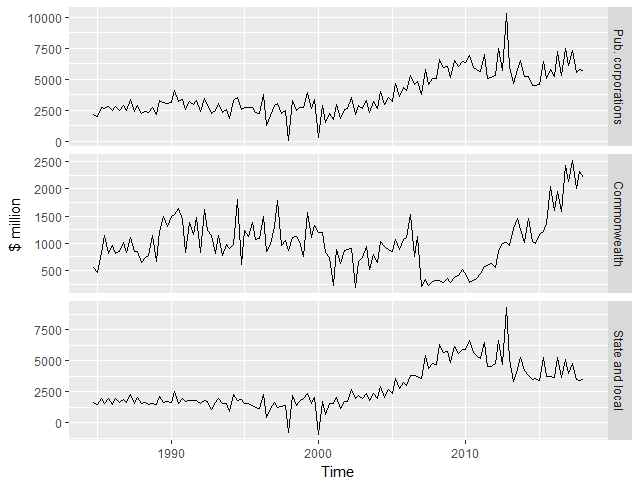
\includegraphics[scale=0.65]{Figs/TS-plots/EXP-hierarchy/set-8.png}
	\caption{Disaggregation of public corporations of Gross fixed capital formations.}\label{EXP-set-8}
\end{figure}

\begin{figure}[H]
 	\centering
 	\small
 	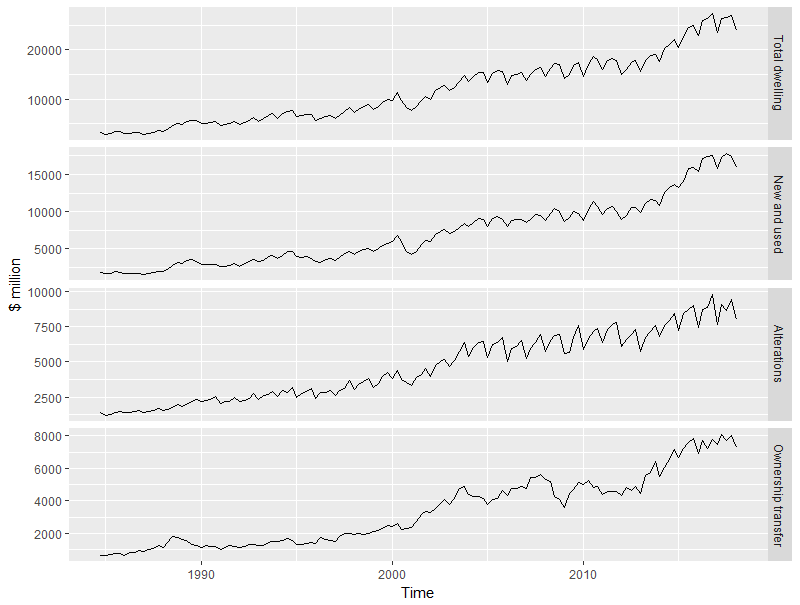
\includegraphics[scale=0.5]{Figs/TS-plots/EXP-hierarchy/set-9.png}
 	\caption{Disaggregation of total dwelling and ownership transfer.}\label{EXP-set-9}
\end{figure}

\begin{figure}[H]
	\centering
	\small
	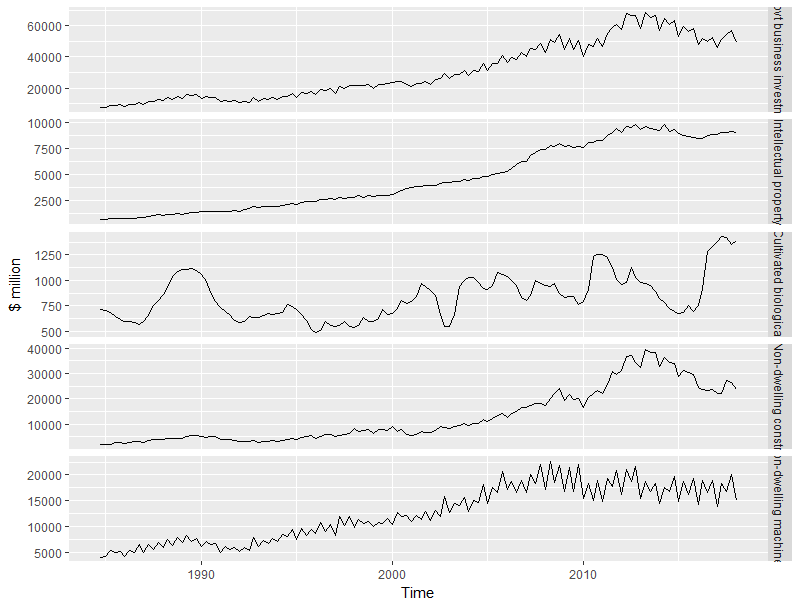
\includegraphics[scale=0.5]{Figs/TS-plots/EXP-hierarchy/set-10.png}
	\caption{Main disaggregation of total private business investments.}\label{EXP-set-10}
\end{figure}

\begin{figure}[H]
	\centering
	\small
	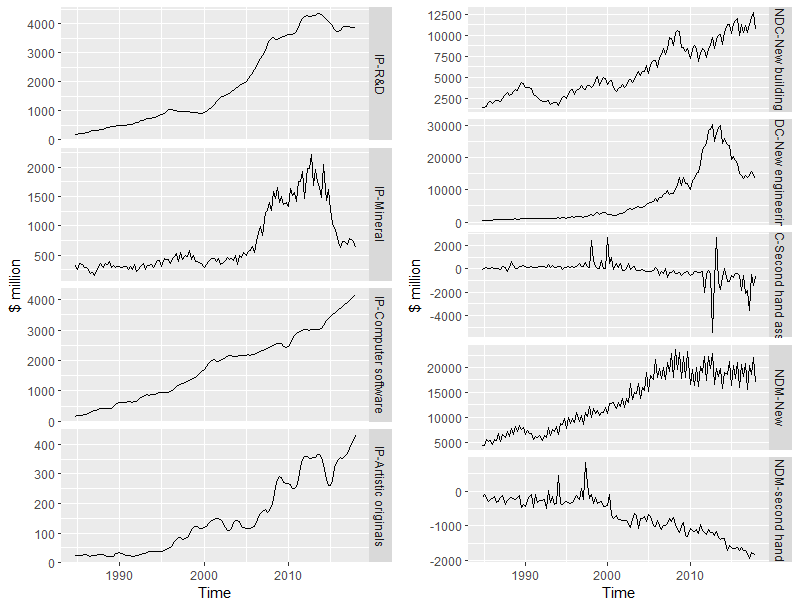
\includegraphics[scale=0.5]{Figs/TS-plots/EXP-hierarchy/set-11.png}
	\caption{Remaining disaggregation of total private business investments.}\label{EXP-set-11}
\end{figure}

\begin{figure}[H]
	\centering
	\small
	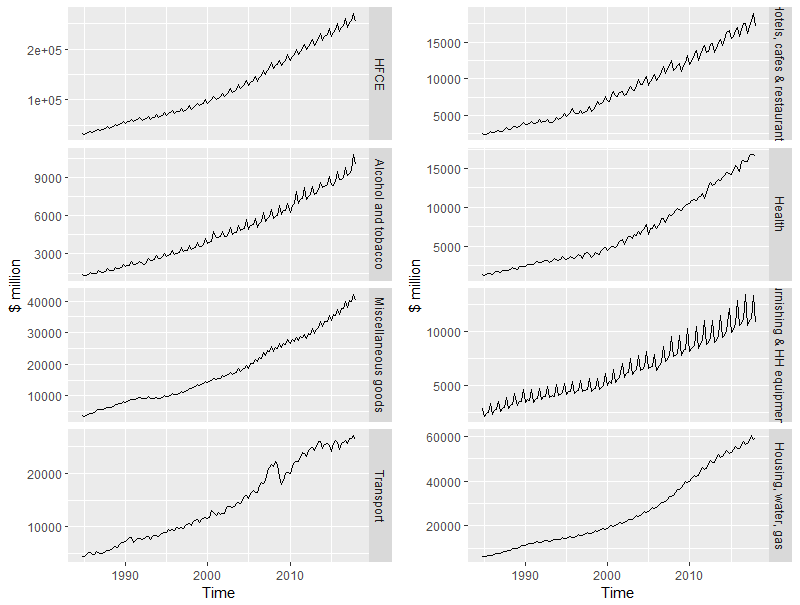
\includegraphics[scale=0.5]{Figs/TS-plots/EXP-hierarchy/set-12.png}
	\caption{Main disaggregation of household final consumption expenditure.}\label{EXP-set-12}
\end{figure}

\begin{figure}[H]
	\centering
	\small
	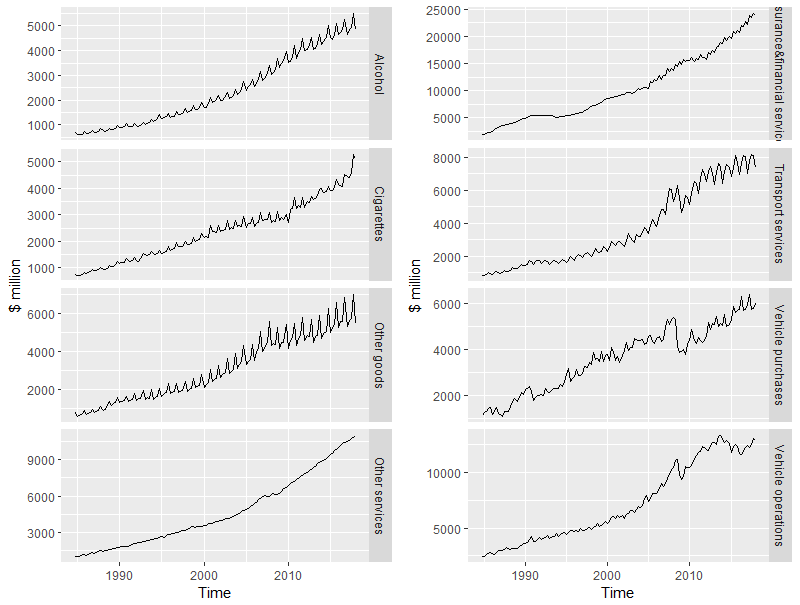
\includegraphics[scale=0.5]{Figs/TS-plots/EXP-hierarchy/set-13.png}
	\caption{Disaggregation of household final consumption expenditure.}\label{EXP-set-13}
\end{figure}

\begin{figure}[H]
	\centering
	\small
	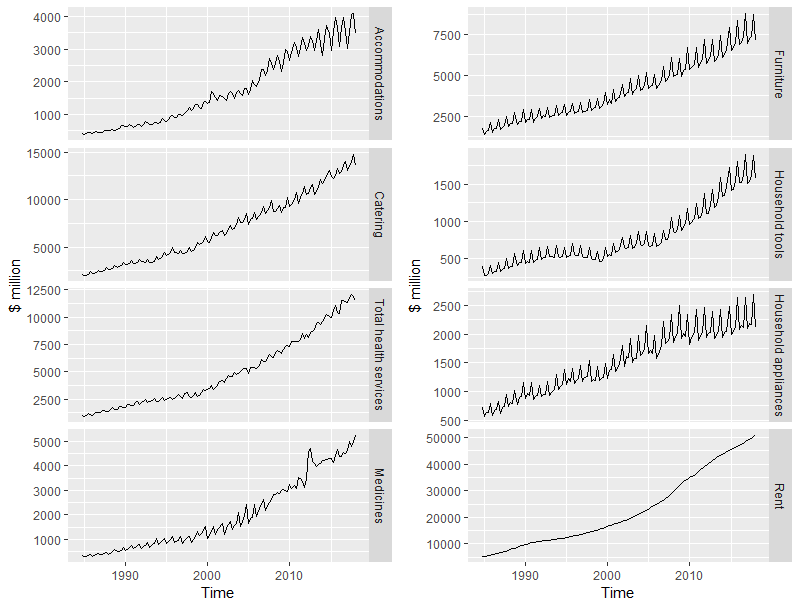
\includegraphics[scale=0.5]{Figs/TS-plots/EXP-hierarchy/set-14.png}
	\caption{Disaggregation of household final consumption expenditure.}\label{EXP-set-14}
\end{figure}

\begin{figure}[H]
	\centering
	\small
	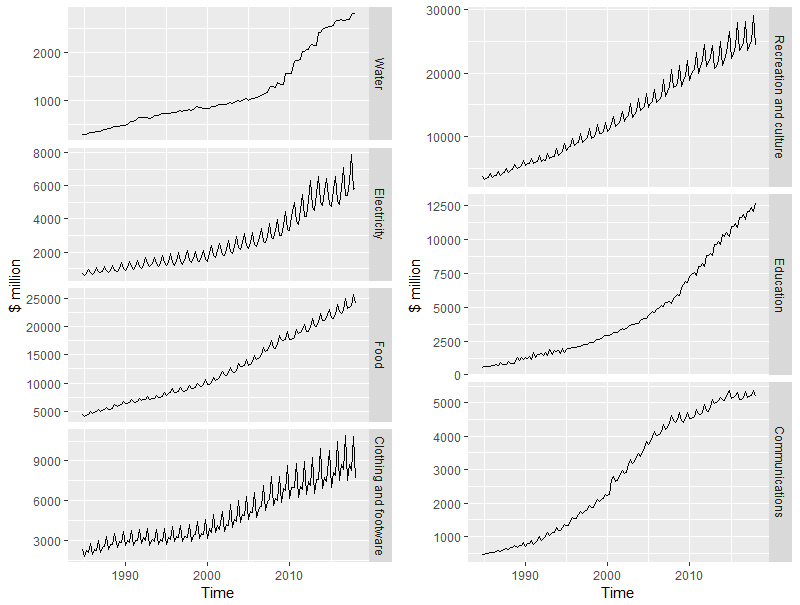
\includegraphics[scale=0.5]{Figs/TS-plots/EXP-hierarchy/set-15.png}
	\caption{Disaggregation of household final consumption expenditure.}\label{EXP-set-15}
\end{figure}

\pagebreak
\bibliographystyle{agsm}

\bibliography{References_BookChapter_HTS,library}


\end{document}
